% \documentclass[german,master,buw]{webisthesis} % Weimar
\documentclass[german,bachelor,fsu]{webisthesis} % Jena
% \documentclass[german,bachelor,ul]{webisthesis} % Leipzig
% \documentclass[german,master,buw,web]{webisthesis} % Weimar, for web page
% \documentclass[german,bachelor,fsu,web]{webisthesis} % Jena, for web page
% \documentclass[german,bachelor,ul,web]{webisthesis} % Leipzig, for web page
%
% Non-default programme
% ---------------------
% \documentclass[english,master,buw]{webisthesis}\global\thesisprogramme{Human-Computer Interaction}
% \documentclass[english,master,buw]{webisthesis}\global\thesisfrontpagefaculty{Faculty of Civil Engineering/Faculty of Media}\global\thesisprogramme{Digital Engineering}
% \documentclass[german,bachelor,buw]{webisthesis}\global\thesisprogramme{Informatik\\Schwerpunkt Medieninformatik}
% \documentclass[german,bachelor,buw]{webisthesis}\global\thesisprogramme{Informatik\\Schwerpunkt Security and Data Science}
%
% When you change the language, pdflatex may halt on recompilation.
% Just hit enter to continue and recompile again. This should fix it.


%
% Values
% ------
%\ThesisSetTitle{Aggregating Pairwise Preferences for Relevance Transfer}
\ThesisSetTitle{Transferring Relevance Judgments with Pairwise Preferences}
%\ThesisSetTitle{Transferring Old Relevance Judgments For Evaluation of Neural Retrieval}
%\ThesisSetTitle{Reusing Old Relevance Judgments to Evaluate Modern Neural Retrieval Models}
%\ThesisSetTitle{Transferring Relevance Judgments from Older to Newer Web Crawls}
%\ThesisSetTitle{Integrating Pairwise Preferences into State-of-the-Art Information Retrieval Systems}
\ThesisSetKeywords{pairwise preferenes, IR} % only for PDF meta attributes
\ThesisSetLocation{Jena 07743, Germany} 

\ThesisSetAuthor{Fabian Hofer}
\ThesisSetStudentNumber{199111}
\ThesisSetDateOfBirth{22}{8}{2002}
\ThesisSetPlaceOfBirth{Eisenach}

% Supervisors should usually be Professors from the candidate's university. A second supervisor is not always needed. 
\ThesisSetSupervisors{Prof.\ Dr.\ Matthias Hagen,Maik Fröbe}

\ThesisSetSubmissionDate{13}{3}{2025}

%
% Suggested Packages
% ------------------
\usepackage[sort&compress]{natbib}
%   Allows citing in different ways (e.g., only the authors if you use the
%   citation again within a short time).
%
\usepackage{booktabs}
%    For tables ``looking the right way''.
%
% \usepackage{tabularx}
%    Enables tables with columns that automatically fill the page width.
%
% \usepackage[ruled,algochapter]{algorithm2e}
%    A package for pseudo code algorithms.
%
% \usepackage{amsmath}
%    For tabular-style formatting of mathematical environments.

\usepackage{rotating} % Add this to the preamble to get rotated tables
\usepackage{bbold}
\usepackage{multirow}
\usepackage{graphics}
\usepackage{tcolorbox}
\usepackage{svg}
\usepackage{longtable}

\usepackage{fontawesome}
%    For lots of awesome glyphs: https://mirror.physik.tu-berlin.de/pub/CTAN/fonts/fontawesome/doc/fontawesome.pdf

%
% Commenting (by your supervisor)
% -------------------------------
\usepackage{xcolor}
\usepackage{soul}
\newcommand{\bscom}[2]{%
  % #1 Original text.
  % #2 Replacement text.
    \st{\scriptsize\,#1}{\color{blue}\scriptsize\,#2}%
  }

% Create links in the pdf document
% Hyperref has some incompatibilities with other packages
% Some other packages must be loaded before, some after hyperref
% Additional options to the hyperref package can be provided in the braces [], like in
% \usehyperref[backref] % This will add back references in the bibliography that some people like ... some don't ... so better ask your supervisor ;-)
\usehyperref[]

\begin{document}
\begin{frontmatter}
\begin{abstract}
\section*{Abstract}

Relevance judgments are essential for evaluating and comparing the effectiveness of information retrieval systems. Traditionally, human assessors manually review query-document pairs to determine relevance judgments. This process is costly, time-consuming, and must be repeated for each new test collection. This thesis addresses this challenge by presenting a method for automatically generating relevance judgments using existing annotated datasets. The proposed approach transfers relevance information from a well-judged source corpus to a subset of documents in a target corpus, enriching it with newly generated judgments. The method employs a pairwise preference approach, where a large language model compares already judged documents from the source corpus with candidate documents from the target corpus. To do this, the model is prompted to determine whether a target document is as relevant to a given query as an already judged source document, resulting in an automatically generated set of relevance judgments for the target corpus. To evaluate the effectiveness of the developed approach, the transfer method is applied to multiple existing test collections that already contain relevance judgments. Each collection serves as both a source and its own target corpus, enabling automatic evaluation by comparing the newly generated judgments with the original ones. Additionally, the approach is tested on \texttt{ClueWeb22/b} as an unjudged target corpus. By leveraging pairwise preference with already judged documents, this approach has the potential to significantly reduce the effort for manual annotation while maintaining high-quality relevance judgments, making scalable enrichment of target corpora possible.

\pagebreak

\section*{Kurzfassung}

Relevanzbewertungen sind für die Evaluierung und den Vergleich der Effektivität von Information Retrieval Systemen von entscheidender Bedeutung. Traditionell werden diese Bewertungen von menschlichen Annotatoren manuell durch die Bewertung von Anfrage-Dokument-Paaren bestimmt. Dieser Prozess ist jedoch zeitaufwändig und muss für jeden neuen Testdatensatz wiederholt werden. Diese Arbeit untersucht, ob der Aufwand für die Erstellung von Relevanzbewertungen reduziert werden kann, indem bestehende annotierte Datensätze zur automatischen Generierung neuer Bewertungen verwendet werden. Dazu wird ein Ansatz vorgestellt, der Relevanzinformationen aus einem gut annotierten Datensatz extrahiert und auf einen neuen Datensatz überträgt. Das Verfahren basiert auf paarweisen Vergleichen. Dazu werden bereits annotierte Dokumente eines Quelldatensatzes mit Dokumenten eines Zieldatensatzes in einem Large Language Model verglichen. Das Modell hat die Aufgabe zu bestimmen, ob ein Zieldokument für eine bestimmte Anfrage genauso relevant ist wie ein bereits bewertetes Quelldokument. Das Ergebnis ist ein automatisch generierter Satz von Relevanzbewertungen für den Zieldatensatz. Zur Evaluierung des Ansatzes wird dieser auf mehrere bestehende Testdatensätze angewendet, die bereits Relevanzbewertungen enthalten. Jede dieser Sammlungen dient sowohl als Quell- als auch als Zieldatensatz, was einen Vergleich der generierten Relevanzbewertungen mit den ursprünglichen Relevanzbewertungen ermöglicht. Zusätzlich wird der Transfer mit \texttt{ClueWeb22/b} als Zieldatensatz getestet. Durch die Nutzung bereits annotierter Dokumente und paarweiser Vergleiche hat dieser Ansatz das Potenzial, den manuellen Annotationsaufwand neuer Datensätze deutlich zu reduzieren und gleichzeitig qualitativ hochwertige Relevanzbewertungen zu generieren.
\end{abstract}

\tableofcontents

% \chapter*{Acknowledgements} % optional
% I thank the authors of the webisthesis template for their excellent work!

% \listoffigures % optional, usually not needed

% \listoftables % optional, usually not needed

% \listofalgorithms % optional, usually not needed
%    requires package algorithm2e

% optional: list of symbols/notation (e.g., using the nomencl package) but usually not needed
\end{frontmatter}

\chapter{Introduction}\label{introduction} 

Static test collections, which consist of information needs, documents, and relevance judgments, are commonly used to evaluate the retrieval effectiveness of retrieval systems \cite{sanderson:2010}. Retrieval effectiveness measures how well a retrieval system retrieves relevant documents to a given information need. To assess this effectiveness, relevance judgments are required to classify the retrieved results as relevant or non-relevant to an information need. However, the use of such static test collections relies on several simplications that are not realistic in practice. One assumption is that information needs, documents, and relevance judgments remain unchanged over time. While information needs are often stable, documents frequently change over time \mbox{\cite{cho:2000}}. This presents a challenge for evaluation methods based on static collections, as relevance judgments made for one version of a document may not apply to later versions.
\\\\
Relevance judgments are assessments made by humans as to whether a document is relevant to a given query. This process is time-consuming and expensive due to human needs. One of the first widely used test collections, the Cranfield test collection \mbox{\cite{cleverdon:91}}, included a small corpus of just $1\,400$ scientific abstracts with 225 queries and manually assigned relevance judgments. While feasible for small collections, judging with human effort becomes impractical when dealing with modern large-scale corpora containing millions or even billions of documents. Due to the large amount of data, only a small subset of documents can be judged anyway. 
\\\\\\\\\\\\\\
In this thesis, I propose an approach for transferring relevance judgments from an existing test collection to a target corpus using pairwise preferences. The goal is to automate the creation of relevance judgments for the target corpus, thereby enriching its set of relevance judgments and enabling more accurate evaluation of retrieval systems on the target corpus. Additionally, this approach aims to reduce the need for human judgment, which would otherwise be \mbox{required} for manually assessing relevance judgments.
\\\\
The transfer pipeline consists of several steps that process the source and target datasets to perform pairwise preference comparisons between documents from both corpora in order to generate new relevance judgments. The pipeline starts with a source dataset that includes a document corpus and an associated retrieval task that provides a set of queries and relevance judgments for the documents in the corpus.
\\\\
Only documents from the source corpus that have at least one relevance judgment contain information that can be used for relevance transfer. Therefore, an initial document selection is performed on the source document corpus. To enable a more fine-granular comparison, the selected documents are segmented into smaller text passages. This segmentation is necessary because later steps, particularly the pairwise preference evaluation, rely on transformer models, which have a maximum context length they can process. Another advantage of segmenting documents is that relevant information is typically concentrated in specific parts of a document rather than being spread throughout. To identify these relevant parts, the resulting passages are ranked to determine the most relevant passages for each query in the retrieval task. The highest-scoring passages are then used in the next step to identify documents from the target corpus that are likely to be relevant to the query and should therefore be judged. The same segmentation approach is applied to the selected candidate documents from the target corpus.
\\\\
To finally conduct the pairwise preference comparisions, each target passage is paired with the most relevant passages from the source dataset for the corresponding query. A large language model is provided with tuples of the selected canidates, consisting of \texttt{(query, known source passage, target passage to judged)}. The model is prompted to determine the relevance of the target passage to the query based on the known passage. The resulting relevance scores from these pairwise comparisons are then used to generate the final relevance judgments for the target documents. After aggregating the relevance scores, the pipeline outputs a set of relevance judgments for each query in the retrieval task for the selected subset of target documents.
\\\\
The final part of this thesis focuses on evaluating the effectiveness of the relevance transfer pipeline. For this purpose, widely used datasets such as \texttt{Args.me}, \texttt{Disks 4+5}, and \texttt{MS MARCO} serve as source corpora. Their existing retrieval tasks provide the foundation for the transfer process, which is evaluated in two phases. First, the pipeline is applied within the source datasets themselves to assess how accurately the transfer process can reproduce known relevance judgments. To compare the generated relevance judgments with the actual ones, rank correlation is computed between both label sets. This allows for an automated evaluation against the existing relevance judgments of the source datasets. In the second phase, the pipeline is used to transfer relevance judgments from the source datasets to \texttt{ClueWeb22/b}, the selected target corpus. Since this corpus lacks pre-existing relevance judgments, evaluation in this case requires manual assessment. To address this, a representative subset of relevance judgments will be manually assessed for \texttt{ClueWeb22/b} in order to evaluate the quality of the automatically created ones.
\chapter{Related Work}\label{related-work}

The idea of transferring relevance judgments from one dataset to another has been explored in multiple studies. Fr\"{o}be et al.~\cite{froebe:2021} investigated the issue of near-duplicate documents within widely-used web crawls such as \texttt{ClueWeb} and \texttt{Common Crawl}. The authors proposed a deduplication approach to address this issue and, as an extension, explored the potential of transferring relevance judgments between near-duplicate documents. However, their study also emphasized that newly collected judgments remain necessary for evaluating retrieval systems on newer datasets. An example of ineffective relevance judgment transfer was conducted on the  \texttt{MS MARCO} corpus. The \mbox{\texttt{MS MARCO} crawl} is a widely used training and test dataset in information retrieval, available both as a document corpus and as a passage corpus. Fr\"{o}be et al.~\cite{froebe:2022} analyzed  why retrieval models trained on \texttt{MS MARCO v1} performed better than those trained on \texttt{MS MARCO  v2}. In version one, the passage dataset was available and judged before the document dataset. To take advantage of this, relevance judgments were directly transferred from the passage dataset to the document dataset by assigning the same relevance judgment to any document that had the same URL as the judged passage. A similar process was applied to enrich version two, where documents were assigned the same relevance judgment as their corresponding documents from version one if they had the same URL. The issue with this approach was that the document corpus in version one was crawled one year after the passage corpus, during which time the content of URLs remained largely unchanged. However, the document corpus in version two was crawled four years after the passage corpus, leading to many content changes. This dissimilarity resulted in inaccurate relevance transfers. This example highlights the importance of considering document content when transferring relevance judgments between datasets. To address this challenge, the transfer pipeline in this thesis employs a pairwise preference approach to compare old and new documents, ensuring a more reliable transfer of relevance information.
\\\\
A more automated approach to infer relevance judgments was introduced by MacAvaney and Soldaini~\cite{macavaney:2023}, who proposed One-Shot Labelers ($\mathbb{1}$SL) to predict relevance for unjudged passages using nearest neighbor searches and various prompting strategies. Their goal was to examine the potential of large language models to fill \glqq holes\grqq{} (i.e., unjudged documents) in relevance assessments for information retrieval evaluations. Their results demonstrated that instruction-tuned models, such as \texttt{FLAN-T5} \cite{chung:2022}, can provide reliable relevance estimations. However, their study focused only on passages and left document level inference as future work. This thesis addresses that gap by employing a pairwise inference approach with \texttt{FLAN-T5} to generate \mbox{labels at document level}.
\\\\
Re-ranking methods play a crucial role in improving document ranking effectiveness. Traditional approaches include pointwise, pairwise, and listwise ranking, each with a trade-off between efficiency and effectiveness. Pradeep et al.~\cite{pradeep:2021} introduced a multi-stage ranking framework that combines document expansion, pointwise ranking, and pairwise re-ranking to enhance retrieval performance. Their findings showed that pairwise ranking models, such as \texttt{DuoT5}, significantly improve ranking quality, even in zero-shot scenarios. Inspired by this, the relevance transfer pipeline in this thesis leverages pairwise inference to determine the relevance of documents in the target corpus.
\\\\
One of the key challenges in the relevance transfer pipeline is the selection of candidate documents from the target corpus for relevance transfer. The selection is a critical step, as it determines which documents should be considered for relevance inference. MacAvaney et al.~\cite{macavaney:2022} highlighted a major limitation in re-ranking pipelines. They depend on the recall of the initial candidate pool, meaning that documents not retrieved in this initial stage cannot be re-ranked later. To address this issue, they proposed a graph-based adaptive re-ranking approach, which expands the candidate pool beyond the initial retrieval set by leveraging the clustering hypothesis \mbox{\cite{jardine:1971}}. This hypothesis states that closely related documents are often relevant to the same queries. Following this idea, this thesis explores various nearest neighbor strategies for selecting documents for relevance transfer.
\\\\\\\\\\\\\\
Processing pairwise preferences can be computationally expensive, particularly when dealing with large document collections, since it requires evaluating $k^2-k$ preferences for $k$ documents. To save computing resources, Gienapp et al.~\cite{gienapp:2022} investigated whether sampling from all possible preference pairs could improve the efficiency of pairwise re-ranking models without sacrificing effectiveness. Their findings showed that re-ranking effectiveness could be maintained with only one-third of the usual comparisons, with only a minor performance drop when further reducing comparisons. Based on that, the number of pairwise comparisons in the relevance transfer pipeline must not be exhaustive to maintain effective. Similarly, Zhuang et al.~\cite{zhuang:2024} introduced \glqq Setwise prompting \grqq{}, a novel zero-shot document ranking approach designed to reduce the number of required inferences while balancing efficiency and effectiveness. Their results demonstrated the advantages of Setwise prompting over traditional pairwise methods, suggesting that it could serve as a more fine-grained alternative for pairwise inference in relevance transfer.
\\\\
Overall, these studies provide essential insights into relevance transfer, candidate retrieval, and efficiency optimizations, forming the foundation for the relevance transfer pipeline developed in this thesis.
\chapter{Methodology}\label{methodology}

In this Chapter, I present the individual steps of the pipeline used to process the datasets. I begin by introducing all the datasets on which the transfer process was performed and evaluated. Subsequently, I discuss each step of the processing pipeline in detail. The goal is to automatically infer \texttt{qrels} for the target dataset through pairwise preferences based on the existing \texttt{qrels} of the source dataset.
\\\\
The first step in the processing pipeline involves segmenting a selection of documents in the source dataset into passages. Relevant information within a document, if present, is typically confined to specific parts and not in the whole document. To improve the results in the pairwise preferences later, the goal is on filtering out only those passages that are highly relevant to a query.
\\\\
The second step identifies the passages of a document that are most relevant to the query of its \texttt{qrel}. For each \texttt{qrel} in the source dataset, i.e., the \texttt{(query, document, label)} triples, all passages of the document are treated as individual queries and submitted as requests against the source dataset. Based on the responses to these requests, various metrics are calculated to measure the proportion of relevant documents retrieved in the document ranking. Passages containing a large amount of relevant information for the query of the \texttt{qrel} retrieve more relevant documents and achieve better metrics than those contributing little or no information to the query.

\pagebreak

In the third step, the quality of the assigned passage scores is evaluated using different rank correlation methods. Based on the evaluation results, the metric with the highest rank correlation is used to select candidates for the pairwise preferences. In this selection phase, documents, referred to as candidates, are identified in the target dataset for which \texttt{qrels} will be determined. A candidate, similar to a \texttt{qrel}, consists of a query $q$, a candidate $c$, a set of known, relevant passages, and a set of known, non relevant passages for $q$ from the source dataset. Since the relevant and non relevant passages are later used for the pairwise preference, each candidate $c$ from the target dataset is also divided into passages $c=(c_1, c_2, ..., c_n)$.
\\\\
In the final step, the pairwise preferences are inferred. All candidates, i.e., triples consisting of \texttt{(query text, non/relevant passage text, unknown passage text)}, are fed into a pairwise ranking model to determine whether the unknown passage is as relevant as the known passage concerning the query text. From the results of the pairwise preferences, labels for the respective unknown passages are generated through the aggregation of all pairwise preferences with the known passages. A label for an entire document in the target dataset is then created by aggregating the labels of all its passages.

\pagebreak


% ========
% Datasets
% ========
\section{Datasets}\label{datasets}

\begin{table}[h!]
    \centering
    \footnotesize
    \caption{List of source datasets and their associated retrieval tasks from which existing \texttt{qrels} where transferd into the target dataset \texttt{ClueWeb22/b}.}
    \label{table:datasets}
    \begin{tabular}{crcrrr}
        \toprule
        \multicolumn{2}{c}{\textbf{Corpus}} & \multicolumn{4}{c}{\textbf{ Associated Retrieval Tasks}} \\
        \cmidrule(lr){1-2} \cmidrule(lr){3-6}
        Name & documents  & Name & Queries &\texttt{qrels} & Labels \\
        \toprule
        
        Args.me & 0.4~m & Touché 2020 Task 1 & 49 & 2,298 & 3 \\
        \midrule

        \multirow{4}{*}{ClueWeb09} & \multirow{4}{*}{1.0~b} & TREC 2009 Web Track & 50 & 23,601 & 3 \\
        & & TREC 2010 Web Track & 50 & 25,329 & 4 \\
        & & TREC 2011 Web Track & 50 & 19,381 & 4\\
        & & TREC 2012 Web Track & 50 & 16,055 & 5 \\
        \midrule

        \multirow{4}{*}{ClueWeb12} & \multirow{4}{*}{731.7~m} & TREC 2013 Web Track & 50 & 14,474 & 5 \\
        & & TREC 2014 Web Track & 50 & 14,432 & 5 \\
        & & Touché 2021 Task 2 & 50 & 2,076 & 3 \\
        & & Touché 2022 Task 2 & 50 & 2,107 & 3 \\
        \midrule

        \multirow{3}{*}{Disks4+5} & \multirow{3}{*}{0.5~m} & Robust04 & 250 & 311,410 & 3 \\
        & & TREC-7 & 50 & 80,345 & 2 \\
        & & TREC-8 & 50 & 86,830 & 2 \\
        \midrule

        \multirow{2}{*}{MS MARCO} & \multirow{2}{*}{3.2~m} & TREC 2019 DL Track & 43 & 16,258 & 4 \\
        & & TREC 2020 DL Track & 45 & 9,098 & 4 \\
        
        \bottomrule
    \end{tabular}
\end{table}

To simplify data handling, I used \texttt{ir\_datasets}~\citep{macavaney:2021}, a Python package that provides numerous datasets and their associated retrieval tasks. The advantage of \texttt{ir\_datasets} is that it provides a standardized interface for accessing data. Using various iterators, the package manages access to corpora, queries, and \texttt{qrels}, enabling the processing pipeline to handle different datasets in a uniform way. The datasets and retrieval tasks used in this research are listed in Table~\ref{table:datasets}. The source datasets were selected because they are widely used in the field of information retrieval and because each dataset comes up with associated retrieval tasks in \texttt{ir\_datasets}. The retrieval tasks, providing \texttt{qrels} for the source datasets, are later transferd to the target dataset, \texttt{ClueWeb22/b}. The target dataset, \texttt{ClueWeb22/b}, was chosen because it is currently the newest ClueWeb corpus in the \texttt{Lemur Project}\footnote{https://lemurproject.org}. The corpus is significantly large, containing over 1.0~billion documents. Due to its size, the ratio of \texttt{qrels} to documents is relatively low. Therefore, the goal is to transfer the existing \texttt{qrels} from the source datasets and their associated retrieval tasks to generate new \texttt{qrels} for \texttt{ClueWeb22/b}, thereby enriching the corpus with additional relevance judgments. 


% =====================
% Document Segmentation
% =====================
\section{Document Segmentation}\label{document-segmentation}

After selecting the datasets and their associated retrieval tasks, including the queries and \texttt{qrels}, the first step in the processing pipeline is the segmentation of documents from the source datasets into passages. This step was done because the relevance of a document is often confined to specific sections rather than the entire text. By segmenting documents into passages, the pipeline can focus solely on the relevant passages, disregarding non-relevant parts of a document in the subsequent processing.

% Document Selection
\subsection{Document Selection}\label{document-selection}

Instead of segmenting the entire source dataset, only a selection of documents is needed. The workflow begins by selecting only already judged documents from the source dataset. A document is considered judged if it contains at least one relevance assessment in the \texttt{qrels} of the associated retrieval task. Only these documents are suitable for relevance transfer, as their relevance has already been determined. Documents without relevance judgments are excluded, as they provide no usable information for the transfer procedure.
\\\\
As shown in Table~\ref{table:datasets}, the number of possible relevance label values varies across retrieval tasks. Some tasks use binary labels, such as \textit{"not relevant"} (label 0) and \textit{“relevant”} (label 1). Others employ a Likert scale, distinguishing between levels such as \textit{“relevant”} and \textit{“highly relevant”}. Tasks with additional gradations for non relevant \texttt{qrels}, such as \textit{"not relevant"} (label 0) and \textit{"negatively relevant”} (label -1), were standardized during processing. Labels smaller than 0 were mapped to \textit{"not relevant"} (label 0). \textcolor{red}{This standardization was applied because the metrics used in this study, e.g., \texttt{precision@10}, do not differentiate between different levels of not relevant}.
\\\\
So far, all documents with at least one relevance assessment for any query of the retrieval task are identified. For each query and each possible label value in the retrieval task, all documents matching the query-label combination are determined. These documents are then assigned to the corresponding query-label pairs. Large retrieval tasks, such as Robust04 with over 300,000~\texttt{qrels}, contain many documents for each query-label pair. Therefore, the number of documents per query-label pair is limited. The pairs are used to identify for each query the label with the fewest docuemtns. The number of documents for each query-label pair is then set to the determined minimum, up to a maximum of 50 documents. 
\\\\
This limit reduces processing effort while ensuring that only a representative subset of judged documents is used for relevance transfer. The reason for limiting the number of documents per label for each query to the minimum frequency per query-label combination is to standardize the number of representative documents per label for each query. This avoids that the relevance transfer is biased towards a specific label in the transfer process.

% Segmentation with spaCy
\subsection{Segmentation with spaCy}\label{segmentation-with-spacy}

Once the documents are selected, they are segmented into passages to facilitate further processing. For this purpose, the GitHub repository grill-lab/trec-cast-tools\footnote{https://github.com/grill-lab/trec-cast-tools} was utilized. This repository provides a suite of scripts specifically designed for processing TREC CAst tracks. Among its features is a wrapper class for document segmentation that leverages the capabilities of the \texttt{spaCy}\footnote{https://spacy.io} library, a powerful tool for Natural Language Processing (NLP) in Python.
\\\\
The segmentation workflow employs \texttt{spaCy's} SentenceRecognizer\footnote{https://spacy.io/api/sentencerecognizer} component, which divides text into sentences. First, the wrapper class uses the SentenceRecognizer pipeline to split the documents into sentences. Then, the returned sentences from \texttt{spaCy} are concatenated into passages, each limited to a maximum size of 250 words. As a result, each document is transformed into a series of uniquely identifiable passages. These identifiers consist of the original document ID combined with an additional passage ID, ensuring traceability throughout the processing pipeline.
\\\\
The documents from the source dataset, selected in the first step, are now available as uniquely passages. In the next stage of the processing pipeline, these individual passages are classified. In cases where a document is judged as relevant to a query, the relevant information is often dispersed throughout the text. To address this, the processing pipeline identifies the passages with a high density of relevant information. This step is essential for optimizing the results of the pairwise preferences in the final stage. It ensures that the most relevant and non-relevant passages are accurately identified for each query.


% ===============
% Passage Scoring
% ===============
\section{Passage Scoring}\label{passage-scoring}

In the first step of the processing pipeline, a subset of the documents from the corpus was segmented into passages. Only documents with at least one relevance assessment in the \texttt{qrels} of the retrieval task were considered for selection. This was done to transfer the information from existing relevance assessments in subsequent stages of the pipeline. To determine which passages of a document best reflect the relevance label from a \texttt{qrel}, i.e., \texttt{(query, document, relevance)} triple, and which passages are most relevant to a query, a ranking of the individual passages is performed in this step.
\\\\
As detailed in Section~[\nameref{selection-documents}], each query-label combination of the retrieval task has an associated set of \texttt{qrels}. To evaluate all passages of the selected documents associated to a query-label combination, the following procedure is applied. First, each passage of a selected document is treated independently and submitted as a query to the source dataset. Then, based on the retrieved ranking of documents for this query, the relevance of the passage is computed using \texttt{precision@10} and \texttt{nDCG@10}.
\\\\
\textbf{Precision} is the fraction of retrieved documents that are relevant to the requested information. In this context, the requested information is the query of the \texttt{qrel} of the retrieval task to which the document is assigned, regardless of whether the document is labeled relevant or non-relevant to the query. Restricting the evaluation to \texttt{precision@10} ensures that only the top 10 retrieved documents are considered. The result of this evaluation is assigned as a score to the query-passage combination.
\\\\
\textbf{Normalized Discounted Cumulative Gain} (\texttt{nDCG}) is another metric commonly used in information retrieval to evaluate the quality of a ranking. Cumulative Gain (\texttt{CG}) represents the sum of all relevance labels for the retrieved document ranking. Again, the query of the retrieval task to which the document is assigned serves for determining the labels of the retrieved documents. Unlike \texttt{precision}, \texttt{CG} considers the label values instead of simply differentiating between non-relevant and relevant labels. This provides greater granularity in retrieval tasks with more than two labels, enabling more nuanced scoring of the passages of a document. The advanced Discounted Cumulative Gain (\texttt{DCG}) further refines this evaluation. It introduces a positional factor to the ranking. It assigns higher weight to relevant results that appear earlier in the ranking. The final score, \texttt{nDCG}, is calculated by normalizing the \texttt{DCG} score with the \texttt{Ideal DCG} (\texttt{IDCG}), which represents the optimal theoretical ranking for the query. As for \texttt{precision}, the evaluation is limited to the first 10 documents by calculating \texttt{nDCG@10}.
\\\\
Passages with a high density of information relevant to a inforamtion need are theoretically more likely to retrieve relevant documents and  for that achieve higher scores on the metrics described above. Conversely, passages that contribute minimal or no relevant information to a inforamtion need result in lower scores due to fewer retrieved relevant documents.
\\\\
Since this study does not aim to optimize or analyze a specific set of retriever systems but uses them for passage scoring, a diverse selection of models was employed to minimize bias in the scores that could arise from relying on a single model. For that reason \texttt{Precision} and \texttt{nDCG} scores were calculated using the following retriever systems: \texttt{BM25, DFR\_BM25, DFIZ, DLH, DPH, DirichletLM, Hiemstra\_LM, LGD, PL2, and TF\_IDF}. An evaluation of which model best scores the passages in relation to the goal of relevance transfer follows in Chapter~\ref{evaluation}~[\nameref{rank-correlation-passage-scores}].
\\\\
In this pipeline stage, the individual passages of the selected documents belonging to the query-label pairs were scored. These scores will be the basis for the subsequent steps to identify candidates from the target dataset. The selected candidates will get new relevance assessments inferred at the end of the pipeline. Furthermore, these scores will determine the known passages from the source dataset, used in pairwise preferences alongside the candidates.


% ====================
% Candidate Retreiaval
% ====================
\section{Candidate Selection}\label{candidate-selection}

This section outlines the methods used to select candidates for the pairwise preference inference. A candidate consists of a passage from the source dataset, a passage from the target dataset, and a query from a retrieval task, i.e. \texttt{(source passage, target passage, query)}. The goal is to score each candidate using pairwise preferences to infer new relevance assessments for a set of target documents. The process begins with selecting document with retrieval from the target dataset.

% Document Retrieval from Target Dataset
\subsection{Document Retrieval from Target Dataset}\label{document-retrieval-from-target-dataset}

For each query in a retrieval task of a source dataset, a set of documents from the target dataset is retrieved. The aim is to identify documents most likely to be relevant to the query. For that, all strategies employ \texttt{BM25} model for retrieval due to its simplicity and efficiency \textcolor{red}{REF\_PAPER}. Since this step only requires a preliminary selection of potentially relevant documents, \texttt{BM25} is sufficient for this task. A fine-grained relevance classification is performed later through the pairwise preferences. Chapter~\ref{evaluation}~[\nameref{candidate-selection}] evaluates these strategies to assess their effectiveness in identifying relevant documents.
\\\\
\textbf{Naive Approach}
The first approach, termed \texttt{naive}, involves submitting each query from the retrieval task to the target dataset corpus to generate a ranking of potentially relevant documents. From this ranking, the top 1000 documents are initially assigned as candidates. Unfortunately, some search queries include ambiguities, leaving room for interpretation regarding the intended information. For example, the query \textit{``Apple``} could refer to either the technology brand or the fruit. To address such ambiguities, the query description of each query is included in the retrieval process. A query description is a brief text that provides additional context, clarifying the search intent and specifying the query's focus. The query description is treated as an independent query and also submitted to the corpus, retrieving an additional top 1000 documents based on the BM25 ranking. After filtering out duplicates between the two sets, up to 2000 unique documents per query are selected for further processing.
\\\\
\textbf{Nearest Neighbor Approach}
The second approach, \texttt{nearest neighbor}, builds on the relevant documents identified in the initial pipeline step descripted in Chapter~\ref{methodology}~[\nameref{document-selection}]. The passages of all selected documents of a query are now used as independent queries to retrieve documents from the target dataset. From the resulting rankings, the top 20 documents are added to the candidate set for the corresponding query. This process is repeated for all passages of all relevant documents. As a result, each passage can contribute up to 20 unique documents to the candidate set.
\\\\
\textbf{Union Approach}
The third approach, called \texttt{union}, combines the \texttt{naive} and \texttt{nearest neighbor} approaches into a single candidate set for each query. This combination is intended to enhance the \texttt{Recall} of the number of retrieved relevant docuements by including a broader set of potentially relevant documents. However, the increased number of documents may reduce \texttt{Precision} by including more irrelevant entries, thereby increasing the workload for pairwise preference evaluations in later stages. The \texttt{Recall} and \texttt{Precision} of the approaches are evaluated in Chapter~\ref{evaluation}~[\nameref{candidate-selection}].

% Postprocessing of Selected Target Documents
\subsection{Postprocessing of Selected Target Documents}\label{postprocessing-of-selected-target-documents}
As described in Section~\nameref{segmentation-with-spacy}, selected documents from the source dataset are segmented into passages for later processing. Since pairwise preferences will be applied at passage level, documents from both the source and target datasets have to be divided into passages. This is done using the same process as outlined before. First, \texttt{spaCy} is employed for segmenting the chosen target documents into sentences, and then passages are formed by concatenating sentences.

% Composing Final Candidates
\subsection{Composing Final Candidates}
As mentioned before, a candidate comprises a passage from the source dataset, a passage from the target dataset, and a query provided by a retrieval task. The queries are provided by the retrieval task which is used to facilitate the transfer of its existing \texttt{qrels}. The documents from the target dataset, along with their associated passages, are identified as just described. To conduct pairwise preference comparisons, passages from the source dataset need to be selected. The objective is to compare each selected passage from the target dataset for a given query against 15 relevant and 5 non-relevant passages from the source dataset corresponding to the same query. To determine the relevant and non-relevant passages, the computed scores of the previous pipeline stage, Section~\nameref{passage-scoring}, are used. The selection is made using two different strategies referred to as \texttt{simple selection} and \texttt{diversified selection}.
\\\\
\textbf{Simple Selection}
During the \nameref{passage-scoring} stage, each selected passage from the source dataset is evaluated and assigned scores based on the \texttt{precision@10} and \texttt{nDCG@10} metrics. These scores are now used to generate a ranking for each query. Following this strategy, the 15 highest-scoring passages and the 5 lowest-scoring passages for each query are selected.
\\\\
\textbf{Diversified Selection}
It is possible that the top- and lowest-rated passages are predominantly drawn from a small subset of documents. While such passages may satisfy the selection criteria of the \texttt{simple selection}, this concentration could lead to unintended side effects by limiting variation in the pairwise preferences. To mitigate potential bias because of reduced document diversity, this approach restricts the selection to a maximum of one passage per document. Specifically, it selects the top 15 and bottom 5 passages for each query, ensuring that each passage is sourced from a distinct document. This strategy enhances diversity in pairwise preference comparisons by incorporating a wider range of source documents.
\\\\
For each query, 20 selected passages from either the \texttt{simple} or \texttt{diversified selection} approach are carried forward to the final pipeline stage. These candidates will go through pairwise preference evaluations to infer new relevance assessments for the selected target dataset documents.

% ====================
% Pairwise Preferences
% ====================
\section{Pairwise Preferences}\label{pairwise-transfering-relevance-labels-across-datasets}

To transfer relevance labels from the old dataset to the new dataset, the DuoT5 transformer model was utilized. This model takes a query and two documents as input and outputs a relevance score, which represents the probability that the first document is more relevant than the second. Here, a "document" refers to a passage. To assign a relevance label to a passage in the new dataset, it is compared against the top 20 to 30 passages for the same query in the old dataset. Pairwise comparison results and their associated queries are cached to avoid redundant calculations, and the final relevance score is determined by averaging the pairwise results. Two approaches are used to select passages for comparison, as detailed below.

\subsection{Pairwise Preferences Approach 1}\label{pairwise-preferences-approach-1}

This approach identifies 20 to 30 passages from the old dataset most relevant to the query for which the new passage is being labeled. To prevent biases from comparing passages within the same document, all passages from the same document as the first passage are excluded. The first passage is the highest-scoring passage from its document, the second passage is the next highest-scoring passage from another document, and so on. The relevance score for the new passage is then calculated by averaging the scores from pairwise comparisons with the selected top passages.

\subsection{Pairwise Preferences Approach 2}\label{pairwise-preferences-approach-2}

This approach is similar to the first but employs an additional step to eliminate overlaps with the same document. After selecting the highest-scoring passage for a query, the retrieval scores for all passages are recomputed, excluding the document of the already-selected passage from the retrieved documents. This ensures no passages from the same document are used more than once in the comparison. As with the first approach, the final relevance score is obtained by averaging the pairwise comparison scores between the new passage and the top 20 to 30 passages from the old dataset.
\chapter{Evaluation}\label{evaluation}

This chapter focuses on the evaluation of the transfer pipeline. First, the individual steps of the pipeline are analyzed and evaluated to examine intermediate results and identify potential weaknesses, starting with an assessment of the scores assigned to the selected passages from the source datasets. Next, the different approaches for selecting candidate documents from the target document corpus are evaluated to determine the most effective approach.
\\\\
The evaluation of the candidate retrieval approaches can only be conducted by applying the transfer pipeline to a target dataset that already contains query relevance judgments. This is necessary because the goal of the candidate retrieval is to pre-select candidate documents from a target corpus that are likely to be relevant to a query. To measure this accurately, the target documents must be labeled with existing relevance judgments.
\\\\
The second part of the chapter focuses on the evaluation of the inferred relevance judgments through two transfer strategies. The first evaluation applies the transfer pipeline to a source dataset and uses the same dataset as the target. This self-transfer evaluation measures how well the pipeline reproduces known relevance judgments within the same dataset. The second evaluation assesses the final transfer to \texttt{ClueWeb22/b} as the target dataset. To facilitate this evaluation, a pooling process is conducted on the candidate documents selected by the best-performing candidate retrieval approach. This is followed by a manual relevance judgment of the pooled documents. The quality of the transferred relevance judgments to \texttt{ClueWeb22/b} is then evaluated based on these manual relevance judgments.
% ================
% Rank Correlation
% ================
\section{Rank Correlation}\label{rank-correlation}

\begin{table}[t]
  \centering
  \caption{Comparison of rank correlation metrics computed by Kendall's $\tau$ and Spearman's $\rho$. The table shows the rank correlation between the reference scores $[0.2,0.7,0.5]$ and three label sets: two with an expected correlation of $1$, and one with lower correlation. Default represents the actual rank correlation scores, while Greedy shows the scores obtained by greedily mapping the reference scores to the label set, representing the idealized rank correlation outcome.}
  \label{tab:rank-correlation}
  \begin{tabular}{ccccc}
      \toprule
      \textbf{Comparative Set} & \multicolumn{2}{c}{\textbf{Default}} & \multicolumn{2}{c}{\textbf{Greedy}} \\
      \cmidrule(lr){2-3} \cmidrule(lr){4-5}
                               & $\tau$ & $\rho$ & $\tau$ & $\rho$ \\
      \midrule
      
      $[0, 2, 1]$ & 1.00 & 0.99  & 1.00  & 1.00 \\
      $[0, 1, 1]$ & 0.82 & 0.92  & 1.00  & 1.00 \\
      $[0, 0, 1]$ & 0.00 & 0.11  & 0.50  & 0.50 \\
      \bottomrule
  \end{tabular}
\end{table}

Before starting with the evaluation of the transfer pipeline, I present the metrics used to evaluate the relevance judgments produced by the pipeline against the actual relevance judgments provided by the retrieval tasks. This clarification is important, as the evaluation results of the passage scores \mbox{(Section~\ref{passage-scoring})} and the final relevance judgments (Section~\ref{pairwise-preferences}) generated by the transfer pipeline are based on these metrics.
\\\\
\texttt{Inter-Annotator Agreement}~\citep{artstein:2017} is a statistical measure that quantifies the consistency among multiple annotators when labeling the same dataset. It provides insight into annotation quality by indicating the level of agreement or disagreement over all annotations. However, this measure requires all annotators to use the same categorical label set. In this thesis, retrieval tasks assign integer relevance labels ($\in \mathbb{N}$), while the inferred relevance labels are continuous scores ($\in \mathbb{R}^{+}$). Due to this mismatch, the \mbox{\texttt{Inter-Annotator Agreement}} is unsuitable for evaluation.
\\\\
Instead, \texttt{Rank Correlation} is used to compare actual relevance labels with the inferred relevance scores. \texttt{Rank Correlation} evaluates how well two rankings align. Here, the retrieval task's relevance judgments serve as the ground truth, against which the transfer pipeline's inferred judgments are compared. The correlation metrics used are \texttt{Kendall's $\tau$} and \texttt{Spearman's $\rho$}. Both metrics compute the rank correlation between linear orders~\citep{monjardet:1998}, making them well-suited for the retrieval task labels and inferred scores. A high rank correlation indicates that the generated judgments preserve the ranking order of the original relevance labels, what is the goal.
\\\\
Table~\ref{tab:rank-correlation} illustrates how these metrics assess sample relevance judgments. It presents agreement between example reference scores $[0.2, 0.7, 0.5]$ and three label sets: the first two yielding an expected correlation of $1$, while the third exhibits a lower correlation. The \texttt{Default} column contains correlation scores computed by standard \texttt{Kendall's $\tau$} and \texttt{Spearman's $\rho$} algorithms. Unlike the default algorithms, the goal in this thesis is to maximize alignment between inferred relevance scores and ground truth labels. For instance, the relevance scores $[0.2, 0.7, 0.5]$ should ideally correspond to the label set $[0, 1, 1]$ (second row of Table~\ref{tab:rank-correlation}). This alignment can be achieved by mapping scores less than or equal to $0.2$ to label $0$ and scores greater than $0.2$ to label $1$. Therefore, the intended rank correlation for this example should be $1$.
\\\\
To accomplish this, a modified version called \texttt{Greedy} was tested alongside the default algorithms. This variant greedily maps the relevance scores to the label set, producing the highest possible correlation. The example demonstrates that standard correlation metrics are sensitive to the rank order of relevance judgments, whereas the \texttt{Greedy} version eliminates this sensitivity, achieving the maximum correlation scores.

% Before starting with the evaluation of the transfer pipeline, I present the metrics used to evaluate the relevance judgments produced by the pipeline against the actual relevance judgments provided by the retrieval tasks. This clarification is important, as the evaluation results of the passage scores \mbox{(Section~\ref{passage-scoring})} and the final relevance judgments (Section~\ref{pairwise-preferences}) generated by the transfer pipeline are based on these metrics.
% \\\\
% The \texttt{Inter-Annotator Agreement}~\citep{artstein:2017} is a statistical measure that quantifies the consistency between annotations provided by multiple annotators. It indicates the level of agreement or disagreement among annotators when labeling the same dataset, thereby offering insight into the quality of the annotations. In this thesis, the ground truth annotation is represented by the relevance judgments provided by the retrieval tasks. These judgments are compared to the inferred relevance judgments generated by the transfer pipeline. A high \texttt{Inter-Annotator Aggreement} score indicates a strong agreement between the actual relevance labels and the inferred relevance labels.
% \\\\
% Various methods exist for calculating \texttt{Inter-Annotator Aggreement}, each with its strengths and weaknesses. In this thesis, the retrieval tasks provide judgments as integer labels, i.e., $\in \mathbb{N}$, while the inferred relevance labels are represented as actual relevance scores, i.e., $\in \mathbb{R}^{+}$. Consequently, not every correlation method is suitable for computing the aggreement between the relevances. Therefore, the correlation metrics used to evaluate the level of agreement are \texttt{Kendall's $\tau$} and \texttt{Spearman's $\rho$}. Both metrics compute the rank correlation between linear orders~\citep{monjardet:1998}, making them well-suited to the nature of the retrieval tasks labels and inferred relevance scores in this thesis.
% \\\\
% Table~\ref{tab:rank-correlation} presents an example of how the correlation metrics are calculated based on some sample labels of the relevance judgments. The table shows the agreement between example reference scores $[0.2, 0.7, 0.5]$ and three label sets: the first two with an expected correlation of $1$, and the last one with lower correlation. The \texttt{Default} column represents the actual rank correlation scores computed by the standard algorithms of \texttt{Kendall's $\tau$} and \texttt{Spearman's $\rho$}.
% \\\\\\\\\\\\\\
% In contrast to the default algorithms, the desired rank correlation for this thesis, is characterized by the ability to map the inferred relevance scores to the actual relevance labels from the retrieval task in the best possible way. For example, the relevance scores $[0.2, 0.7, 0.5]$ should be perfectly mapped to the label set $[0, 1, 1]$ in the second row of Table~\ref{tab:rank-correlation}. This could be achieved by assuming that all relevance scores smaller equal $0.2$ correspond to label $0$ and all scores greater $0.2$ correspond to label $1$. Therefore, the intended rank correlation for this example should be $1$, in this thesis. To achieve this, a modified variant called \texttt{Greedy} was tested alongside the default versions. This variant greedily maps the reference scores to the label set, representing the idealized rank correlation outcome. This example demonstrates that the default correlation metrics are sensitive to the rank order of the relevance judgments, whereas the \texttt{Greedy} variant avoids this sensitivity, achieving the maximum possible correlation scores.


% ==================
% Document Selection
% ==================
\section{Document Selection}\label{eval-document-selection}

The first step in the transfer pipeline was selecting and segmenting a subset of documents for each query in a retrieval task from the source dataset. These selected documents play a crucial role in two subsequent steps, identifying candidate documents from the target corpus and performing pairwise preference comparisons using \texttt{DouPrompt}. Since only a subset of documents is required per query, two selection criteria were applied. First, only documents with at least one relevance judgment in the \texttt{qrel store} were considered, as documents without judgments do not provide transferable information. Second, a maximum of 50 relevance judgments per relevance label per query, referred to as a query-label combination, was selected to manage computational complexity.
\\\\\\\\\\\\\\\\\\
Table~\ref{tab:document-selection} presents the results of this selection process. On average, close to 50 documents per query-label combination were selected, ensuring a balanced representation of relevant and non-relevant judgments. Ideally, each query should have approximately 50 non-relevant documents and at least 50 relevant ones. All \texttt{TREC} retrieval tasks performed well, providing the maximum number of non-relevant documents per query. Additionally, \texttt{TREC-19 DL} and \texttt{TREC-20 DL} exceeded the \mbox{threshold} of 50 relevant documents per query, ensuring a diverse pool for candidate retrieval and pairwise comparisons. Similarly, \texttt{TREC-7} and \texttt{TREC-8} achieved strong results, with an average of over 40 relevant documents. \texttt{Robust04} contains a substantial number of relevance judgments for its 250 queries, though most are non-relevant. Nonetheless, it maintains a solid average of over 36 relevant documents per query for further processing. The only outlier is \texttt{Touché 20}, which averages just 28 non-relevant and 19 relevant judgments per query.
\\\\
The lower numbers for \texttt{Touché 20} limit the effectiveness of the nearest neighbor candidate retrieval approach and the pairwise preference comparisons. This is due to the low amount of relevance judgments available in the retrieval task. However, given the relatively small size of \texttt{Args.me} (0.4 million documents), the transfer pipeline's results may remain valuable.
\\\\
This intermediate evaluation confirms that the selection process successfully provides an adequate number of documents for subsequent steps in the pipeline. While \texttt{Touché 20} remains useful, its results should be interpreted cautiously due to the lower document count per query.

% The first step in the transfer pipeline was the selection and segmentation of a subset of documents for each query of a retrieval task from the source dataset. The selected documents play a crucial role in two subsequent steps of the pipeline. First, the selection of candidate documents from the target corpus and second the pairwise preference comparison using \texttt{DouPrompt}. Since only a subset of documents is necessary for each query, two selection conditions were applied. First, only documents with at least one relevance judgment in the \texttt{qrel store} of a retrieval task were considered for selection, as documents without relevance judgments do not have information to transfer. Second, a maximum of 50 relevance judgments per relevance label for each query (referred to as a query-label combination) was selected to limit the number of processed documents.
% \\\\
% The results of the selection process under these conditions are presented in Table~\ref{tab:document-selection}. An average close to 50 documents per query-label combination is possible. In order to have a wide selection of relevant and non-relevant judgments, an average close to 50 documents of non relevant judgments, i.e., documents, and close to or over (if the retrieval tasks has multiple levels of relevant) 50 relevant judgments, i.e., documents per query is aimed for. All \texttt{TREC} retrieval tasks achieve very good results, with providing the maximum of possible non relevant documents for each query. Also, \texttt{TREC-19 DL} and \texttt{TREC-20 DL} also reach in sum total over 50 relevant documents per query, thereby providing a wide range of documents for the candidate retreival step and also possiblilites for the pairwise comparisons at the end. \texttt{TREC-7} and \texttt{TREC-8} are also well performing with an average of over 40 documents per query-label combination. \texttt{Robust04} has a very large amount of relevance judgments for its 250 queries, but most of them are non-relevant judgments. Nevertheless, it achieves a good average of over 36 relevant documents to further process. The only outliner is \texttt{Touché 20} which just receives an average of 28 non relevant and 19 relevant judgments.
% \\\\
% The low numbers of \texttt{Touché 20} limit the possibilities for the nearest neighbor candidate retrieval approach and pairwise preferences combination. The low averages are due to the limited number of relevance judgments provided by the retrieval tasks, see Tabel~\ref{tab:datasets}. But due to the small size of \texttt{Args.me} with just $0.4$ million documents, the outcome of the transfer pipeline is still valuable.
% \\\\
% This intermediate evaluation step shows that the selection process is overall successful in providing a sufficient number of documents for the subsequent steps of the transfer pipeline. The outliner \texttt{Touché 20} is still valuable for the evaluation, but the results should be interpreted with caution due to the low number of documents per query.

\begin{table}[t]
  \centering
  \caption{The table presents the results of the candidate selection process, showing for each label of a retrieval task the number of documents per query for each source dataset. A maximum of 50 documents per query-label combination is possible.}
  \label{tab:document-selection}
  \resizebox{\textwidth}{!}{%
  \begin{tabular}{lcccccc}
      \toprule
      \textbf{Docs./Query} & \textbf{Touché 20} & \textbf{Robust04} & \textbf{TREC-7} & \textbf{TREC-8} & \textbf{TREC-19 DL} & \textbf{TREC-20 DL}  \\

      \midrule

      Label 0        & $27.9$ & $50.0$ & $50.0$ & $50.0$ & $ 49.6$ & $ 50.0$ \\
      Label 1        & $ 6.0$ & $32.8$ & $40.2$ & $40.5$ & $ 31.1$ & $ 28.5$ \\
      Label 2        & $13.0$ & $ 3.8$ &    -   &    -   & $ 23.8$ & $ 16.0$ \\
      Label 3        &    -   &    -   &    -   &    -   & $ 11.7$ & $ 10.3$ \\
      \midrule
      \textbf{Total} & $46.9$ & $86.6$ & $90.2$ & $90.5$ & $116.2$ & $104.8$ \\

      \bottomrule
  \end{tabular}}
\end{table}

%\\\\
% The segmentation of the selected documents was performed using the \texttt{trec-cast-tools} GitHub repository\footnote{\url{https://github.com/grill-lab/trec-cast-tools}}, which splits documents into passages of up to 250 words in length. This segmentation process is independent of the transfer pipeline and is therefore not evaluated in this thesis.
\pagebreak

% ===============
% Passage Scoring
% ===============
\section{Passage Scoring}\label{eval-passage-scoring}

\begin{table}[t]
    \centering
    \caption{Average rank correlations between the assigned passage scores and the original relevance judgments across all queries of a retrieval task, reported using Kendall's $\tau$ and Spearman's $\rho$.}
    \label{tab:passage-scoring}
    \resizebox{\textwidth}{!}{%
    \renewcommand{\arraystretch}{1.2}
    \begin{tabular}{clcccccccccccccc}
        \toprule
        \multicolumn{2}{c}{\textbf{Retrieval Model}} & \multicolumn{2}{c}{\textbf{Touché 20}} & \multicolumn{2}{c}{\textbf{Robust04}} & \multicolumn{2}{c}{\textbf{TREC-7}} & \multicolumn{2}{c}{\textbf{TREC-8}} & \multicolumn{2}{c}{\textbf{TREC-19 DL}} & \multicolumn{2}{c}{\textbf{TREC-20 DL}} & \multicolumn{2}{c}{\textbf{Avg.}} \\
        \cmidrule(lr){3-4} \cmidrule(lr){5-6} \cmidrule(lr){7-8} \cmidrule(lr){9-10} \cmidrule(lr){11-12} \cmidrule(lr){13-14} \cmidrule(lr){15-16}
                                                   & & $\tau$ & $\rho$ & $\tau$ & $\rho$ & $\tau$ & $\rho$ & $\tau$ & $\rho$ & $\tau$ & $\rho$ & $\tau$ & $\rho$ & $\tau$ & $\rho$ \\
        \midrule
        \multirow{10}{*}{\rotatebox{90}{\texttt{ndcg@10}}}
            & BM25         & 0.802 & 0.871 & 0.823 & 0.907 & 0.801 & 0.896 & 0.813 & 0.906 & 0.725 & 0.831 & 0.755 & 0.846 & 0.787 & 0.876 \\
            & DFR\_BM25    & 0.804 & 0.874 & 0.822 & 0.907 & 0.800 & 0.896 & 0.813 & 0.906 & 0.727 & 0.833 & 0.755 & 0.846 & 0.787 & 0.877 \\
            & DFIZ         & 0.778 & 0.852 & 0.820 & 0.906 & 0.796 & 0.896 & 0.800 & 0.898 & 0.730 & 0.836 & 0.753 & 0.845 & 0.780 & 0.872 \\
            & DLH          & 0.839 & 0.901 & 0.831 & 0.913 & 0.810 & 0.903 & 0.825 & 0.915 & 0.735 & 0.839 & 0.754 & 0.845 & 0.799 & 0.886 \\
            & DPH          & 0.783 & 0.856 & 0.820 & 0.905 & 0.799 & 0.895 & 0.809 & 0.903 & 0.725 & 0.831 & 0.753 & 0.844 & 0.782 & 0.872 \\
            & DirichletLM  & 0.679 & 0.752 & 0.816 & 0.902 & 0.798 & 0.896 & 0.802 & 0.898 & 0.721 & 0.825 & 0.751 & 0.841 & 0.761 & 0.852 \\
            & Hiemstra\_LM & 0.855 & 0.914 & 0.829 & 0.912 & 0.807 & 0.902 & 0.819 & 0.910 & 0.729 & 0.834 & 0.759 & 0.849 & \textbf{0.800} & \textbf{0.887} \\
            & LGD          & 0.801 & 0.874 & 0.819 & 0.905 & 0.799 & 0.897 & 0.802 & 0.899 & 0.730 & 0.835 & 0.757 & 0.848 & 0.785 & 0.876 \\
            & PL2          & 0.805 & 0.873 & 0.826 & 0.909 & 0.804 & 0.898 & 0.822 & 0.913 & 0.727 & 0.833 & 0.757 & 0.848 & 0.790 & 0.879 \\
            & TF\_IDF      & 0.807 & 0.876 & 0.823 & 0.907 & 0.801 & 0.896 & 0.814 & 0.907 & 0.726 & 0.832 & 0.755 & 0.847 & 0.788 & 0.877 \\
        \midrule
        \multirow{10}{*}{\rotatebox{90}{\texttt{precision@10}}}
            & BM25         & 0.765 & 0.828 & 0.807 & 0.881 & 0.792 & 0.872 & 0.807 & 0.885 & 0.657 & 0.756 & 0.697 & 0.785 & 0.754 & 0.835 \\
            & DFR\_BM25    & 0.768 & 0.833 & 0.806 & 0.880 & 0.791 & 0.870 & 0.807 & 0.884 & 0.658 & 0.757 & 0.696 & 0.785 & 0.754 & 0.835 \\
            & DFIZ         & 0.729 & 0.798 & 0.801 & 0.874 & 0.785 & 0.863 & 0.791 & 0.869 & 0.661 & 0.760 & 0.695 & 0.784 & 0.744 & 0.824 \\
            & DLH          & 0.802 & 0.862 & 0.817 & 0.889 & 0.803 & 0.881 & 0.823 & 0.899 & 0.666 & 0.764 & 0.697 & 0.785 & \textbf{0.768} & \textbf{0.847} \\
            & DPH          & 0.745 & 0.814 & 0.803 & 0.876 & 0.787 & 0.867 & 0.801 & 0.878 & 0.659 & 0.758 & 0.697 & 0.785 & 0.749 & 0.830 \\
            & DirichletLM  & 0.640 & 0.705 & 0.796 & 0.868 & 0.785 & 0.863 & 0.791 & 0.867 & 0.652 & 0.750 & 0.691 & 0.778 & 0.726 & 0.805 \\
            & Hiemstra\_LM & 0.819 & 0.880 & 0.813 & 0.886 & 0.799 & 0.878 & 0.815 & 0.892 & 0.658 & 0.757 & 0.699 & 0.786 & 0.767 & 0.846 \\
            & LGD          & 0.765 & 0.833 & 0.800 & 0.873 & 0.787 & 0.866 & 0.792 & 0.870 & 0.659 & 0.758 & 0.697 & 0.785 & 0.750 & 0.831 \\
            & PL2          & 0.766 & 0.829 & 0.811 & 0.885 & 0.796 & 0.876 & 0.819 & 0.896 & 0.656 & 0.755 & 0.698 & 0.786 & 0.758 & 0.838 \\
            & TF\_IDF      & 0.769 & 0.832 & 0.808 & 0.881 & 0.793 & 0.872 & 0.808 & 0.885 & 0.657 & 0.756 & 0.697 & 0.785 & 0.755 & 0.835 \\

        \bottomrule
    \end{tabular}}
    \renewcommand{\arraystretch}{1.0}
\end{table}

The next step in the transfer pipeline was to assign relevance scores to the passages of the selected documents from the previous step. This was done to identify the most relevant passages of a document with respect to the actual query associated with a document's relevance judgment. To achieve this, each passage was treated as an independent query and used to retrieve a document ranking from its original source corpus. Based on the retrieved document rankings, \texttt{precision@10} and \texttt{nDCG@10} were computed and assigned as passage scores. Since this study does not aim to optimize or analyze specific retriever systems but rather utilizes them for passage scoring, a diverse selection of models was tested, as listed in Table~\ref{tab:passage-scoring}.
\\\\
To evaluate the quality of the assigned passage scores and determine which retrieval model and metric combination were most effective in determining the relevance of passages, the rank correlation between the original relevance judgments and the newly assigned scores was computed using Kendall's $\tau$ and Spearman's $\rho$. For each retriever-metric combination, an overall document score was aggregated from its passage scores by selecting the maximum passage score. The rank correlation was then computed for all judged \mbox{documents} of each query individually, rather than across all relevance judgments of a retrieval task simultaneously, and then averaged. Macro-averaging across all queries is intended to reduce the effect of potential outliers for individual queries.
% \\\\
% To ensure a robust evaluation of the assigned passage scores, a 5-fold cross-validation was applied across the metrics, aggregation methods, and transformation methods for each combination of retrieval model and retrieval task. First, queries within each retrieval task were divided into five equal subsets (folds). For each fold, one subset was designated as the validation set, while the remaining four subsets formed the training set. In each iteration of the cross-validation, the metric, aggregation method, and transformation method that achieved the highest average correlation score on the training set (four-fifths of the queries) were selected. This selection process involved computing the average correlation score across all queries in the training set for each combination. The chosen combination was then evaluated on the test set (the remaining fifth of the queries) to obtain a final correlation score for that iteration. This process was repeated for all five folds, ensuring that each query subset served as the validation set exactly once. The final cross-validation score for each retrieval model and retrieval task was computed as the average correlation score across all five folds, thereby reducing the impact of overfitting and providing a more reliable estimate of passage scoring performance.
\\\\
The results in Table~\ref{tab:passage-scoring} show that all retrieval models achieved a very high rank correlation across all tested information retrieval tasks. While \texttt{Hiemstra\_LM} was the best-performing model, all models demonstrated strong performance based on the average $\tau$ and $\rho$ values. Therefore, the choice of retrieval model is not a critical factor for subsequent steps in the transfer pipeline, as all models produced passage scores with high rank correlation to the actual relevance labels from the retrieval tasks. This finding also applies to the \texttt{greedy} variant of both rank correlation methods, as shown in Table~\ref{tab:app:passage-scoring}. Although the greedy variant resulted in slightly higher rank correlation scores than the standard version, the overall behavior remained consistent.
\\\\
However, the choice of metric had a significant impact. \texttt{precision@10} consistently resulted in lower rank correlation compared to \texttt{nDCG@10}. This outcome was expected, as \texttt{precision@10} lacks the granularity needed to effectively differentiate between individual passages. Consequently, \texttt{nDCG@10} is the better metric for passage scoring. In the following steps of the transfer pipeline, the passage scores assigned by \texttt{nDCG@10} alongside the retrieval model that achieved the highest rank correlation for each retrieval task is therefore used.
\pagebreak


% ===================
% Candidate Selection
% ===================
\section{Candidate Selection}\label{eval-candidate-selection}

\begin{table}[t]
    \centering
    \footnotesize
    \caption{Overview of recall (Rec.) and the average number of candidate documents per query (Docs.) for all three candidate retrieval approaches, tested with document selection restricted to one passage per document (opd.) and without restriction (def.). The \texttt{Nearest Neighbor} and the \texttt{Union} approaches were also evaluated with varying $k$, determining the number of passages used for candidate retrieval.}
    \label{tab:candidate-selection}
    \resizebox{\textwidth}{!}{%
    \renewcommand{\arraystretch}{1.2}
    \begin{tabular}{ccrcrcrcrcrcrcr}
        \toprule

        \multicolumn{3}{c}{\textbf{Approach}} & \multicolumn{2}{c}{\textbf{Touché 20}} & \multicolumn{2}{c}{\textbf{Robust04}} & \multicolumn{2}{c}{\textbf{TREC-7}} & \multicolumn{2}{c}{\textbf{TREC-8}} & \multicolumn{2}{c}{\textbf{TREC-19 DL}} & \multicolumn{2}{c}{\textbf{TREC-20 DL}} \\

        \cmidrule(lr){4-5} \cmidrule(lr){6-7} \cmidrule(lr){8-9} \cmidrule(lr){10-11} \cmidrule(lr){12-13} \cmidrule(lr){14-15}
                                          & & $k$ & Rec. & Docs. & Rec. & Docs. & Rec. & Docs. & Rec. & Docs. & Rec. & Docs. & Rec. & Docs. \\
        \midrule
        \multirow{2}{*}{\rotatebox{90}{\textbf{Naive}}} & \multirow{2}{*}{-} & \multirow{2}{*}{-} & \multirow{2}{*}{$0.912$} & \multirow{2}{*}{$1\,556$} & \multirow{2}{*}{$0.777$} & \multirow{2}{*}{$1\,572$} & \multirow{2}{*}{$0.657$} & \multirow{2}{*}{$1\,600$} & \multirow{2}{*}{$0.713$} & \multirow{2}{*}{$1\,566$} & \multirow{2}{*}{$0.736$} & \multirow{2}{*}{$976$} & \multirow{2}{*}{$0.751$} & \multirow{2}{*}{$955$} \\
        & & & & & & & & & & & & & & \\

        \midrule
        \multirow{6}{*}{\rotatebox{90}{\textbf{Nearest Neighbor}}} & \multirow{3}{*}{def.} &  10 & $0.609$ &  $97$ & $0.530$ &  $88$ & $0.430$ &  $85$ & $0.449$ &  $89$ & $0.560$ &  $81$ & $0.616$ &  $83$ \\
                                                                                        &  &  50 & $0.828$ & $318$ & $0.744$ & $334$ & $0.696$ & $349$ & $0.665$ & $356$ & $0.872$ & $268$ & $0.906$ & $269$ \\
                                                                                        &  & 100 & $0.978$ & $479$ & $0.833$ & $618$ & $0.787$ & $657$ & $0.757$ & $684$ & $0.966$ & $436$ & $0.974$ & $407$ \\
       \cmidrule(lr){2-15}
                                                                   & \multirow{3}{*}{opd.} &  10 & $0.699$ & $104$ & $0.584$ &  $96$ & $0.495$ &  $99$ & $0.489$ & $101$ & $0.560$ &  $81$ & $0.616$ &  $83$ \\
                                                                                        &  &  50 &   \boldmath$1.0$ & $209$ & $0.876$ & $360$ & $0.826$ & $419$ & $0.797$ & $439$ & $0.872$ & $268$ & $0.906$ & $269$ \\
                                                                                        &  & 100 &   \boldmath$1.0$ & $209$ & $0.885$ & $375$ & $0.826$ & $419$ & $0.797$ & $439$ & $0.966$ & $436$ & $0.974$ & $407$ \\

        \midrule
        \multirow{6}{*}{\rotatebox{90}{\textbf{Union}}} & \multirow{3}{*}{def.} &  10 & $0.931$ & $1\,577$ & $0.855$ & $1\,618$ & $0.771$ & $1\,651$ & $0.795$ & $1\,611$ & $0.859$ & $1\,018$ & $0.856$ &    $996$ \\
                                                                             &  &  50 & $0.948$ & $1\,678$ & $0.906$ & $1\,807$ & $0.861$ & $1\,860$ & $0.860$ & $1\,813$ & $0.954$ & $1\,146$ & $0.958$ & $1\,132$ \\
                                                                             &  & 100 & $0.992$ & $1\,774$ & $0.934$ & $2\,052$ & $0.904$ & $2\,134$ & $0.895$ & $2\,100$ & $0.988$ & $1\,278$ & $0.990$ & $1\,245$ \\
        \cmidrule(lr){2-15}
                                                        & \multirow{3}{*}{opd.} &  10 & $0.935$ & $1\,575$ & $0.865$ & $1\,622$ & $0.792$ & $1\,659$ & $0.808$ & $1\,621$ & $0.859$ & $1\,018$ & $0.856$ &    $996$ \\
                                                                             &  &  50 &   \boldmath$1.0$ & $1\,610$ & $0.950$ & $1\,827$ & \boldmath$0.915$ & $1\,916$ & \boldmath$0.919$ & $1\,888$ & $0.954$ & $1\,146$ & $0.958$ & $1\,132$ \\
                                                                             &  & 100 &   \boldmath$1.0$ & $1\,610$ & \boldmath$0.951$ & $1\,839$ & \boldmath$0.915$ & $1\,916$ & \boldmath$0.919$ & $1\,888$ & \boldmath$0.988$ & $1\,278$ & \boldmath$0.990$ & $1\,245$ \\

        \bottomrule 
    \end{tabular}}
    \renewcommand{\arraystretch}{1.0}
\end{table}

The next step in the transfer pipeline involved selecting documents from the target corpus in order to create new relevance judgments for each query. The goal is to identify documents highly likely to be relevant to a given query. This is crucial, as generating judgments for every query-document pair would be computationally expensive and unnecessary as unjudged documents in a test collection are mostly interpreted as not relevant by default.
\\\\
To maximize the number of likely relevant documents, three selection approaches were tested. The \texttt{Naive} approach retrieved the top 1000 documents from the target corpus using the query text and, when available, a query's narrative for an additional 1000 documents. The \texttt{Nearest Neighbor} approach used the top-scoring passages identified in Section~\ref{passage-scoring} as independent queries to retrieve the top 20 documents from the target corpus as candidates. This approach was tested with different numbers of top passages per query: 10, 50, and 100. Additionally, it was tested with and without a restriction that limited each query's top passages to a maximum of one passage per document. The \texttt{Union} approach combined all documents retrieved by the \texttt{Naive} and each \texttt{Nearest Neighbor} approaches, filtering out duplicate candidates.
\\\\
A recall evaluation of the candidate selection approaches is only possible for the relevance transfer within the same dataset, meaning from a source dataset to its own document corpus. This constraint is because existing relevance judgments must be available for the same retrieval task, i.e., for the same queries, in both the source and target datasets. Consequently, Table~\ref{tab:candidate-selection} presents recall and the average number of candidate documents per query of the transfer pipeline within the same dataset. The recall metric is computed as the proportion of retrieved candidate documents that are judged as relevant relative to the total number of relevant documents in the retrieval task.
\\\\
The \texttt{Naive} approach achieved very high recall for \texttt{Touché 20}, benefiting from its relatively small document corpus (\texttt{Args.me}, 0.4 million documents) and the retrieval of up to 2000 documents per query. However, its performance reduces significantly on all other datasets, because of much larger corpora. Additionally, \texttt{TREC-19 DL} and \texttt{TREC-20 DL} do not provide query narratives, limiting retrieval to a maximum of 1000 documents per query and thereby reducing recall. Overall, the \texttt{Naive} approach was able to retrieve a large amount of relevant documents, but this comes at the cost of including many non-relevant candidates, making the selection less efficient.
\\\\
The \texttt{Nearest Neighbor} approach outperformed \texttt{Naive} in nearly all variants, except when using only the top 10 passages, limiting candidate documents per query to 200. For \texttt{TREC-7} and \texttt{TREC-8}, the number of selected documents did not increase between the \texttt{opd.} top 50 and top 100 variants due to the document selection process evaluated in Section~\ref{eval-document-selection}. As shown in Table~\ref{tab:document-selection}, these retrieval tasks have only one positive relevance label and are restricted to a maximum of 50 relevant documents per query. Thus, using the top 100 passages did not improve recall, as no additional relevant passages available under the \texttt{opd.} constraint. For \texttt{Touché 20}, which has two positive relevance labels, a similar effect was observed due to its overall low number of relevance judgments. However, even if \texttt{Robust04} averages 36 relevant documents, some queries exceed 50 relevant judgments in total, which explains the higher recall achieved with the \texttt{opd.\ 100} variant. Another expected outcome of Table~\ref{tab:candidate-selection} is that the same recall is achieved for \texttt{TREC-19 DL} and \texttt{TREC-20 DL} for the \texttt{def.} and \texttt{opd.} variants. This is because their document corpora consist solely of passages, making the restriction of one passage per document ineffective. Overall, a key finding is that restricting the top passages to a maximum of one passage per document (\texttt{opd.}) consistently improved performance compared to allowing multiple passages per document (\texttt{def.}). This result shows enforcing greater document diversity leads to more effective candidate selection. 
\\\\
The \texttt{Union} approach further improved recall, particularly for \texttt{Robust04}, \texttt{TREC-7}, and \texttt{TREC-8}, where it increased recall by approximately 10 percentage points. For \texttt{TREC-19 DL} and \texttt{TREC-20 DL}, the \texttt{Union (opd.\ 100)} variant improved recall by three percentage points compared to \texttt{Union (opd.\ 50)}, reaching an impressive recall of approximately $99~\%$. However, this improvement came at the cost of tripling or quadrupling the number of retrieved documents per query. Despite this increase, the trade-off remains acceptable, as recall is consistently high across all six tasks, and the number of retrieved documents per query remains below 2000. Therefore, \texttt{Union (opd.\ 100)} is the most effective candidate selection approach and is used in the subsequent step of the pipeline.

% ====================
% Pairwise Preferences
% ====================
\section{Pairwise Preferences}\label{eval-pairwise-preferences}

The candidate selection process, evaluated in Section~\ref{eval-candidate-selection}, identified \linebreak \mbox{\texttt{Union (opd.\ 100)}} as the most effective approach for pre-selecting likely relevant documents from the target corpus. Consequently, the evaluation in this section is conducted using the candidate documents selected by this approach. For further processing with large language models, all candidate documents were segmented into passages, following the same document segmentation \mbox{procedure} as described in Section~\ref{segmentation-with-spacy}.
% The candidate selection process, evaluated in Section~\ref{eval-candidate-selection}, identified \linebreak \mbox{\texttt{Union (opd.\ 100)}} as the most effective approach for pre-selecting likely relevant documents from the target corpus. Therefore, the evaluation in this section is conducted on the candidate documents of this approach. For further processing with large language models, all candidate documents were segmented into passages, exactly as in the document segmentation step in Section~\ref{segmentation-with-spacy}.
\\\\
For each query in a retrieval task, all passages from the selected candidate documents were paired with the 15 most relevant and 5 least relevant passages for that query. These 20 passages were determined through the passage-scoring step described in Section~\ref{passage-scoring}. As evaluated in Section~\ref{eval-passage-scoring}, the passage scores were derived from the retriever-metric combination with the highest rank correlation, ensuring the selection of the 15 highest-scoring relevant and the 5 lowest-scoring non-relevant passages per query. Since Section~\ref{eval-candidate-selection} showed that nearest neighbor approaches performed better when limited to selecting at most one passage per document, this restriction was also applied when selecting the 20 passages, as outlined in Section~\ref{composing-final-candidates} under \texttt{Diversified Selection}.
% For each query in a retrieval task, all passages from the selected candidate documents were paired with the 15 most relevant and 5 most non-relevant passages for that query. These 20 passages were determined using the passage-scoring step described in Section~\ref{passage-scoring}. Based on the evaluation in Section~\ref{eval-passage-scoring}, the passage scores from the retriever-metric combination with the highest rank correlation were used to select the 15 highest-scoring relevant passages and the 5 lowest-scoring non-relevant passages per query. Since the evaluation in Section~\ref{eval-candidate-selection} demonstrated that nearest neighbor approaches with a restriction of at most one passage per document performed better than those without this limitation, the same restriction was applied when selecting the 20 passages, as described in Section~\ref{composing-final-candidates} \texttt{Diversified Selection}.
\\\\
To determine the relevance of candidate documents from the target corpus, tuples consisting of \texttt{(query, known passage, passage to judge)}, were processed using various versions of Google's \texttt{T5} model, Figure~\ref{fig:pairwise-preferences}. For each tuple, the model was prompted to predict the relevance of the target passage to the query, based on the known source passage. After processing all comparisons, each target passage received 20 relevance scores, one for each comparison to a selected source passage. To derive an overall passage score, these individual scores were aggregated and transformed using different methods. The tested aggregation methods included \texttt{mean, min, max, sum}, while the transformation methods included \texttt{id, log, exp, sqrt}. Finally, the relevance score of a document was determined by taking the maximum of all its passage scores.
% To determine relevance for candidate documents from the target corpus, tuples consisting of \texttt{(query, known source passage, target passage to judge)} were processed using various versions of Google's \texttt{T5} model. For each tuple, the model was prompted to predicted the relevance of the target passage in relation to the query, based on the known passage. After doing all comparisons, each target passage received 20 relevance scores, one for each comparison to a selected source passage. To get an overall passage score, all passage scores of the same passage were aggregated and transformed using various methods. Tested aggregation methods are \texttt{mean, min, max, sum} and transformation methods are \texttt{id, log, exp, sqrt}. The final document relevance score was then assigned by taking the maximum of all its passage scores.
\\\\
For comparison, a pointwise approach was tested alongside the pairwise preference approach. In this setup, the \texttt{T5} models received only the query and the target passage, without comparisons to known passages, and was prompted to determine the passage's relevance to the query. Since this approach evaluated each passage independently, no aggregation or transformation was needed at the passage level. However, to derive the final document relevance score, the maximum of all passage scores for the document was used again.

% Transfer Pipeline to Source Corpus itself
\subsection{Transfer Pipeline on Source Corpora}\label{eval-pairwise-preferences-source}

The evaluated rank correlation scores between the actual relevance labels of the source datasets and the generated relevance scores from the self-transfer are listed in Table~\ref{tab:self-pairwise-preferences}. These scores represent the average rank correlation across all queries for each retrieval task. The rank correlation for each query was computed based on all candidates from the \texttt{Union opd.\ 100} approach that had a relevance judgment in the corresponding retrieval task.
\\\\
Overall, the best aggregation method across all three transformer models was \texttt{min}, which achieved the highest rank correlation across all retrieval tasks, except for \texttt{t5-small} with \texttt{max} aggregation. This result suggests that a passage is only as relevant as its least relevant comparison to the source passages. Additionally, the table shows that applying transformation methods to the aggregated passage scores had no impact on the rank correlation evaluation. This is expected, as tested transformations keep the linear orders of the relevance scores, meaning that applying the same transformation to all aggregated scores has no effect on rank correlation, making the step redundant.
\\\\
One notable outlier is \texttt{Touché 20}, which has two key differences from the other evaluated datasets. First, rank correlation scores using \texttt{t5-small} were higher than those for \texttt{flan-t5-small} and \texttt{flan-t5-base}. Second, the pointwise approach for \texttt{flan-t5-base} achieved the overall best rank correlation for \texttt{Touché 20}. Unlike the other datasets, \texttt{Touché 20} has the smallest document corpus (\texttt{Args.me}) and the fewest relevance judgments per query among all tested retrieval tasks. This leads to the assumption that source dataset sparsity can influence model ranking behavior, potentially causing inconsistencies in rank correlation scores due to few information to transfer.
\begin{table}[ht!]
    \centering
    \footnotesize
    \caption{Rank correlations of the inferred relevance judgements to the original document judgments reported in terms of Kendall's $\tau$ and Spearman's $\rho$.}
    \label{tab:self-pairwise-preferences}
    \resizebox{\textwidth}{!}{%
    \renewcommand{\arraystretch}{1.0}
    \begin{tabular}{cclccccccccccccc}
        \toprule

        \multicolumn{3}{c}{\textbf{Approach}} & \multicolumn{2}{c}{\textbf{Touché 20}} & \multicolumn{2}{c}{\textbf{Robust04}} & \multicolumn{2}{c}{\textbf{TREC-7}} & \multicolumn{2}{c}{\textbf{TREC-8}} & \multicolumn{2}{c}{\textbf{TREC-19 DL}} & \multicolumn{2}{c}{\textbf{TREC-20 DL}} \\
        \cmidrule(lr){4-5} \cmidrule(lr){6-7} \cmidrule(lr){8-9} \cmidrule(lr){10-11} \cmidrule(lr){12-13} \cmidrule(lr){14-15}
                            & & & $\tau$ & $\rho$ & $\tau$ & $\rho$ & $\tau$ & $\rho$ & $\tau$ & $\rho$ & $\tau$ & $\rho$ & $\tau$ & $\rho$ \\
        \midrule
        \multirow{16}{*}{\rotatebox{90}{\makecell{\textbf{Pairwise Preferences} \\ \textbf{flan-t5-base}}}}
        & \multirow{4}{*}{\textbf{mean}}
                  & \textbf{id}   & 0.232 & 0.288 & 0.154 & 0.189 & 0.126 & 0.154 & 0.174 & 0.213 & 0.254 & 0.316 & 0.233 & 0.293 \\
                & & \textbf{log}  & 0.232 & 0.288 & 0.154 & 0.189 & 0.126 & 0.154 & 0.174 & 0.213 & 0.254 & 0.316 & 0.233 & 0.293 \\
                & & \textbf{exp}  & 0.232 & 0.288 & 0.154 & 0.189 & 0.126 & 0.154 & 0.174 & 0.213 & 0.254 & 0.316 & 0.233 & 0.293 \\
                & & \textbf{sqrt} & 0.232 & 0.288 & 0.154 & 0.189 & 0.126 & 0.154 & 0.174 & 0.213 & 0.254 & 0.316 & 0.233 & 0.293 \\
        \cmidrule{2-15}
        & \multirow{4}{*}{\textbf{min}}
                  & \textbf{id}   & \textbf{0.250} & \textbf{0.314} & \textbf{0.169} & \textbf{0.208} & \textbf{0.137} & \textbf{0.167} & \textbf{0.187} & \textbf{0.229} & \textbf{0.311} & \textbf{0.387} & \textbf{0.293} & \textbf{0.366} \\
                & & \textbf{log}  & \textbf{0.250} & \textbf{0.314} & \textbf{0.169} & \textbf{0.208} & \textbf{0.137} & \textbf{0.167} & \textbf{0.187} & \textbf{0.229} & \textbf{0.311} & \textbf{0.387} & \textbf{0.293} & \textbf{0.366} \\
                & & \textbf{exp}  & \textbf{0.250} & \textbf{0.314} & \textbf{0.169} & \textbf{0.208} & \textbf{0.137} & \textbf{0.167} & \textbf{0.187} & \textbf{0.229} & \textbf{0.311} & \textbf{0.387} & \textbf{0.293} & \textbf{0.366} \\
                & & \textbf{sqrt} & \textbf{0.250} & \textbf{0.314} & \textbf{0.169} & \textbf{0.208} & \textbf{0.137} & \textbf{0.167} & \textbf{0.187} & \textbf{0.229} & \textbf{0.311} & \textbf{0.387} & \textbf{0.293} & \textbf{0.366} \\
        \cmidrule{2-15}
        & \multirow{4}{*}{\textbf{max}}
                  & \textbf{id}   & 0.226 & 0.283 & 0.079 & 0.097 & 0.084 & 0.103 & 0.080 & 0.098 & 0.107 & 0.136 & 0.120 & 0.151 \\
                & & \textbf{log}  & 0.226 & 0.283 & 0.079 & 0.097 & 0.084 & 0.103 & 0.080 & 0.098 & 0.107 & 0.136 & 0.120 & 0.151 \\
                & & \textbf{exp}  & 0.226 & 0.283 & 0.079 & 0.097 & 0.084 & 0.103 & 0.080 & 0.098 & 0.107 & 0.136 & 0.120 & 0.151 \\
                & & \textbf{sqrt} & 0.226 & 0.283 & 0.079 & 0.097 & 0.084 & 0.103 & 0.080 & 0.098 & 0.107 & 0.136 & 0.120 & 0.151 \\
        \cmidrule{2-15}
        & \multirow{4}{*}{\textbf{sum}}
                  & \textbf{id}   & 0.232 & 0.288 & 0.154 & 0.189 & 0.126 & 0.154 & 0.174 & 0.213 & 0.254 & 0.316 & 0.233 & 0.293 \\
                & & \textbf{log}  & 0.232 & 0.288 & 0.154 & 0.189 & 0.126 & 0.154 & 0.174 & 0.213 & 0.254 & 0.316 & 0.233 & 0.293 \\
                & & \textbf{exp}  & 0.232 & 0.288 & 0.154 & 0.189 & 0.126 & 0.154 & 0.174 & 0.213 & 0.254 & 0.316 & 0.233 & 0.293 \\
                & & \textbf{sqrt} & 0.232 & 0.288 & 0.154 & 0.189 & 0.126 & 0.154 & 0.174 & 0.213 & 0.254 & 0.316 & 0.233 & 0.293 \\
        \midrule

        \multirow{16}{*}{\rotatebox{90}{\makecell{\textbf{Pairwise Preferences} \\ \textbf{flan-t5-small}}}}
        & \multirow{4}{*}{\textbf{mean}}
                  & \textbf{id}   & 0.232 & 0.299 & 0.067 & 0.082 & 0.065 & 0.079 & 0.082 & 0.101 & 0.175 & 0.220 & 0.132 & 0.165 \\
                & & \textbf{log}  & 0.232 & 0.299 & 0.067 & 0.082 & 0.065 & 0.079 & 0.082 & 0.101 & 0.175 & 0.220 & 0.132 & 0.165 \\
                & & \textbf{exp}  & 0.232 & 0.299 & 0.067 & 0.082 & 0.065 & 0.079 & 0.082 & 0.101 & 0.175 & 0.220 & 0.132 & 0.165 \\
                & & \textbf{sqrt} & 0.232 & 0.299 & 0.067 & 0.082 & 0.065 & 0.079 & 0.082 & 0.101 & 0.175 & 0.220 & 0.132 & 0.165 \\
        \cmidrule{2-15}
        & \multirow{4}{*}{\textbf{min}}
                  & \textbf{id}   & \textbf{0.301} & \textbf{0.388} & \textbf{0.082} & \textbf{0.101} & \textbf{0.080} & \textbf{0.097} & \textbf{0.094} & \textbf{0.115} & \textbf{0.224} & \textbf{0.282} & \textbf{0.179} & \textbf{0.224} \\
                & & \textbf{log}  & \textbf{0.301} & \textbf{0.388} & \textbf{0.082} & \textbf{0.101} & \textbf{0.080} & \textbf{0.097} & \textbf{0.094} & \textbf{0.115} & \textbf{0.224} & \textbf{0.282} & \textbf{0.179} & \textbf{0.224} \\
                & & \textbf{exp}  & \textbf{0.301} & \textbf{0.388} & \textbf{0.082} & \textbf{0.101} & \textbf{0.080} & \textbf{0.097} & \textbf{0.094} & \textbf{0.115} & \textbf{0.224} & \textbf{0.282} & \textbf{0.179} & \textbf{0.224} \\
                & & \textbf{sqrt} & \textbf{0.301} & \textbf{0.388} & \textbf{0.082} & \textbf{0.101} & \textbf{0.080} & \textbf{0.097} & \textbf{0.094} & \textbf{0.115} & \textbf{0.224} & \textbf{0.282} & \textbf{0.179} & \textbf{0.224} \\
        \cmidrule{2-15}
        & \multirow{4}{*}{\textbf{max}}
                  & \textbf{id}   & 0.196 & 0.250 & 0.028 & 0.035 & 0.030 & 0.037 & 0.043 & 0.052 & 0.073 & 0.092 & 0.048 & 0.060 \\
                & & \textbf{log}  & 0.196 & 0.250 & 0.028 & 0.035 & 0.030 & 0.037 & 0.043 & 0.052 & 0.073 & 0.092 & 0.048 & 0.060 \\
                & & \textbf{exp}  & 0.196 & 0.250 & 0.028 & 0.035 & 0.030 & 0.037 & 0.043 & 0.052 & 0.073 & 0.092 & 0.048 & 0.060 \\
                & & \textbf{sqrt} & 0.196 & 0.250 & 0.028 & 0.035 & 0.030 & 0.037 & 0.043 & 0.052 & 0.073 & 0.092 & 0.048 & 0.060 \\
        \cmidrule{2-15}
        & \multirow{4}{*}{\textbf{sum}}
                  & \textbf{id}   & 0.232 & 0.299 & 0.067 & 0.082 & 0.065 & 0.079 & 0.082 & 0.101 & 0.175 & 0.220 & 0.132 & 0.165 \\
                & & \textbf{log}  & 0.232 & 0.299 & 0.067 & 0.082 & 0.065 & 0.079 & 0.082 & 0.101 & 0.175 & 0.220 & 0.132 & 0.165 \\
                & & \textbf{exp}  & 0.232 & 0.299 & 0.067 & 0.082 & 0.065 & 0.079 & 0.082 & 0.101 & 0.175 & 0.220 & 0.132 & 0.165 \\
                & & \textbf{sqrt} & 0.232 & 0.299 & 0.067 & 0.082 & 0.065 & 0.079 & 0.082 & 0.101 & 0.175 & 0.220 & 0.132 & 0.165 \\
        \midrule

        \multirow{16}{*}{\rotatebox{90}{\makecell{\textbf{Pairwise Preferences} \\ \textbf{t5-small}}}}
        & \multirow{4}{*}{\textbf{mean}}
                  & \textbf{id}   & 0.239 & 0.308 & -0.003 & -0.003 & 0.001 & 0.001 & -0.005 & -0.006 & -0.050 & -0.063 & -0.042 & -0.053 \\
                & & \textbf{log}  & 0.239 & 0.308 & -0.003 & -0.003 & 0.001 & 0.001 & -0.005 & -0.006 & -0.050 & -0.063 & -0.042 & -0.053 \\
                & & \textbf{exp}  & 0.239 & 0.308 & -0.003 & -0.003 & 0.001 & 0.001 & -0.005 & -0.006 & -0.050 & -0.063 & -0.042 & -0.053 \\
                & & \textbf{sqrt} & 0.239 & 0.308 & -0.003 & -0.003 & 0.001 & 0.001 & -0.005 & -0.006 & -0.050 & -0.063 & -0.042 & -0.053 \\
        \cmidrule{2-15}
        & \multirow{4}{*}{\textbf{min}}
                  & \textbf{id}   & \textbf{0.320} & \textbf{0.410} & \textbf{0.010} & \textbf{0.013} & \textbf{0.025} & \textbf{0.031} & \textbf{0.008} & \textbf{0.010} & -0.039 & -0.050 & \textbf{-0.019} & \textbf{-0.024} \\
                & & \textbf{log}  & \textbf{0.320} & \textbf{0.410} & \textbf{0.010} & \textbf{0.013} & \textbf{0.025} & \textbf{0.031} & \textbf{0.008} & \textbf{0.010} & -0.039 & -0.050 & \textbf{-0.019} & \textbf{-0.024} \\
                & & \textbf{exp}  & \textbf{0.320} & \textbf{0.410} & \textbf{0.010} & \textbf{0.013} & \textbf{0.025} & \textbf{0.031} & \textbf{0.008} & \textbf{0.010} & -0.039 & -0.050 & \textbf{-0.019} & \textbf{-0.024} \\
                & & \textbf{sqrt} & \textbf{0.320} & \textbf{0.410} & \textbf{0.010} & \textbf{0.013} & \textbf{0.025} & \textbf{0.031} & \textbf{0.008} & \textbf{0.010} & -0.039 & -0.050 & \textbf{-0.019} & \textbf{-0.024} \\
        \cmidrule{2-15}
        & \multirow{4}{*}{\textbf{max}}
                  & \textbf{id}   & 0.115 & 0.150 & -0.002 & -0.002 & -0.002 & -0.002 & -0.004 & -0.005 & \textbf{-0.029} & \textbf{-0.037} & -0.042 & -0.053 \\
                & & \textbf{log}  & 0.115 & 0.150 & -0.002 & -0.002 & -0.002 & -0.002 & -0.004 & -0.005 & \textbf{-0.029} & \textbf{-0.037} & -0.042 & -0.053 \\
                & & \textbf{exp}  & 0.115 & 0.150 & -0.002 & -0.002 & -0.002 & -0.002 & -0.004 & -0.005 & \textbf{-0.029} & \textbf{-0.037} & -0.042 & -0.053 \\
                & & \textbf{sqrt} & 0.115 & 0.150 & -0.002 & -0.002 & -0.002 & -0.002 & -0.004 & -0.005 & \textbf{-0.029} & \textbf{-0.037} & -0.042 & -0.053 \\
        \cmidrule{2-15}
        & \multirow{4}{*}{\textbf{sum}}
                  & \textbf{id}   & 0.239 & 0.308 & -0.003 & -0.003 & 0.001 & 0.001 & -0.005 & -0.006 & -0.050 & -0.063 & -0.042 & -0.053 \\
                & & \textbf{log}  & 0.239 & 0.308 & -0.003 & -0.003 & 0.001 & 0.001 & -0.005 & -0.006 & -0.050 & -0.063 & -0.042 & -0.053 \\
                & & \textbf{exp}  & 0.239 & 0.308 & -0.003 & -0.003 & 0.001 & 0.001 & -0.005 & -0.006 & -0.050 & -0.063 & -0.042 & -0.053 \\
                & & \textbf{sqrt} & 0.239 & 0.308 & -0.003 & -0.003 & 0.001 & 0.001 & -0.005 & -0.006 & -0.050 & -0.063 & -0.042 & -0.053 \\
        \midrule

        \multirow{5}{*}{\rotatebox{90}{\makecell{\textbf{Pointwise} \\ \textbf{Preferences}}}}
            & & & & & & & & & & & & & & \\
            & \multicolumn{2}{c}{\textbf{flan-t5-base}}  & 0.350 & 0.440 & -0.013 & -0.016 & -0.003 & -0.004 & -0.026 & -0.032 & 0.037 & 0.048 & 0.031 & 0.039 \\
            & \multicolumn{2}{c}{\textbf{flan-t5-small}} & -0.127 & -0.162 & -0.011 & -0.014 & -0.001 & -0.001 & -0.018 & -0.022 & -0.048 & -0.061 & -0.031 & -0.040 \\
            & \multicolumn{2}{c}{\textbf{t5-small}}      & -0.152 & -0.194 & 0.004 & 0.005 & 0.013 & 0.015 & 0.005 & 0.006 & -0.056 & -0.070 & -0.042 & -0.053 \\
            & & & & & & & & & & & & & & \\
        \bottomrule 
    \end{tabular}}
    \renewcommand{\arraystretch}{1.0}
\end{table}
\\\\\\
The results of the retrieval tasks based on Disks4+5 and MS MARCO were highly acceptable. In all cases, the most advanced transformer model, \linebreak \texttt{flan-t5-base}, outperformed the other two models in both pairwise and pointwise preference approaches. A key takeaway from this evaluation is that the pointwise preference approach performed poorly across all tested models, yielding almost no correlation between predicted relevance and actual labels. This underscores the limitation of pointwise approaches in predicting document relevance based solely on the document itself. In contrast, the pairwise preference approach achieved notable rank correlation values. Specifically, for \texttt{flan-t5-base}, the retrieval tasks based on the \texttt{Disks4+5} corpus achieved rank correlations ranging from $0.137$ to $0.229$. For the retrieval tasks based on the \texttt{MS MARCO} passage corpus, the inferred relevance scores achieved rank correlations of approximately $0.3$ for Kendall's $\tau$ and $3.7$ for Spearman's $\rho$, indicating a weak to moderate rank correlation.
\\\\
The high correlation scores for \texttt{TREC-DL} 19 and \texttt{TREC-DL 20}, when compared to other datasets, except \texttt{Touché 20}, are likely due to two factors. First, as analyzed in Section~\ref{eval-document-selection}, these retrieval tasks have a relatively high number of judgments per query, providing a strong foundation for relevance transfer. Second, the \texttt{MS MARCO} corpus is a passage corpus, meaning all documents processed by the transfer pipeline were already given as polished passages. As a result, the pairwise comparisons performed the evaluation on individual passages for \texttt{MS MARCO} rather than segmented sections of longer documents. In contrast, the segmentation using \texttt{spaCy}  segments text based on punctuation and maximum passage length which is more rudimentary. Since this work does not include an evaluation of document segmentation methods, the question of optimal document segmentation remains open for future research.
\\\\
The evaluation was also conducted using the \texttt{greedy} versions of Kendall's and Spearman's rank correlations, as shown in Table~\ref{tab:app:self-pairwise-preferences}. Across all datasets, these scores were slightly higher, but the trends observed with the default Kendall and Spearman metrics remained consistent.
\pagebreak
\begin{figure}[ht!]
    \centering
    \begin{tabular}{ccc}
        \textbf{Pairwise Preferences} & \hspace{2cm} & \textbf{Pointwise Preferences} \\
    \end{tabular}
    \footnotesize
    % First row
    \begin{subfigure}[b]{0.49\textwidth}
        \centering
        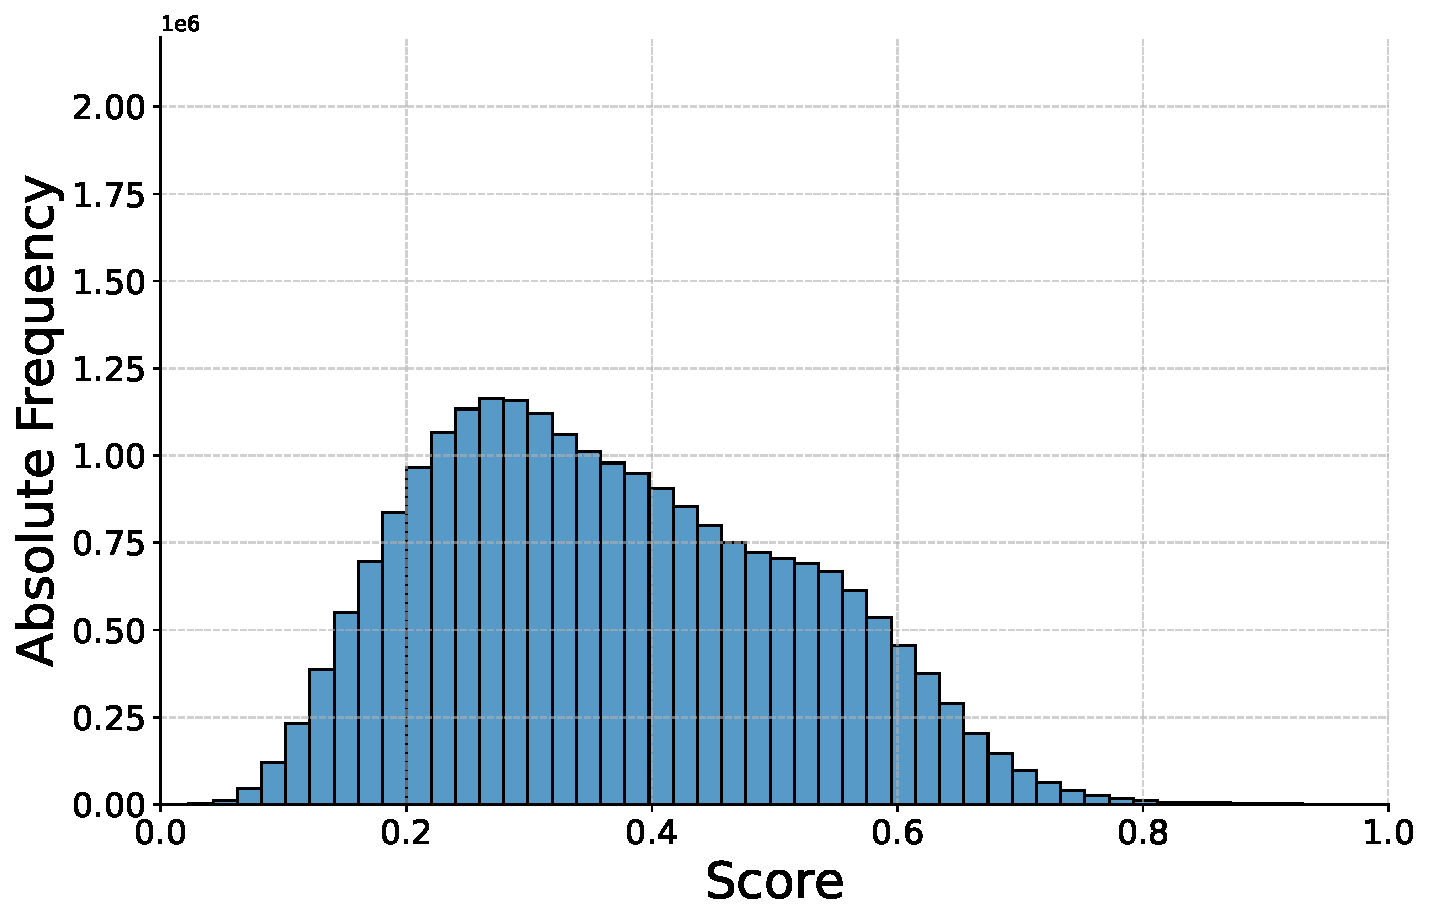
\includegraphics[width=\textwidth]{graphics/evaluation/pairwise_score_distribution_flan-t5-base.pdf}
        \label{fig:pairwise_flan-t5-base}
    \end{subfigure}
    \hfill
    \begin{subfigure}[b]{0.49\textwidth}
        \centering
        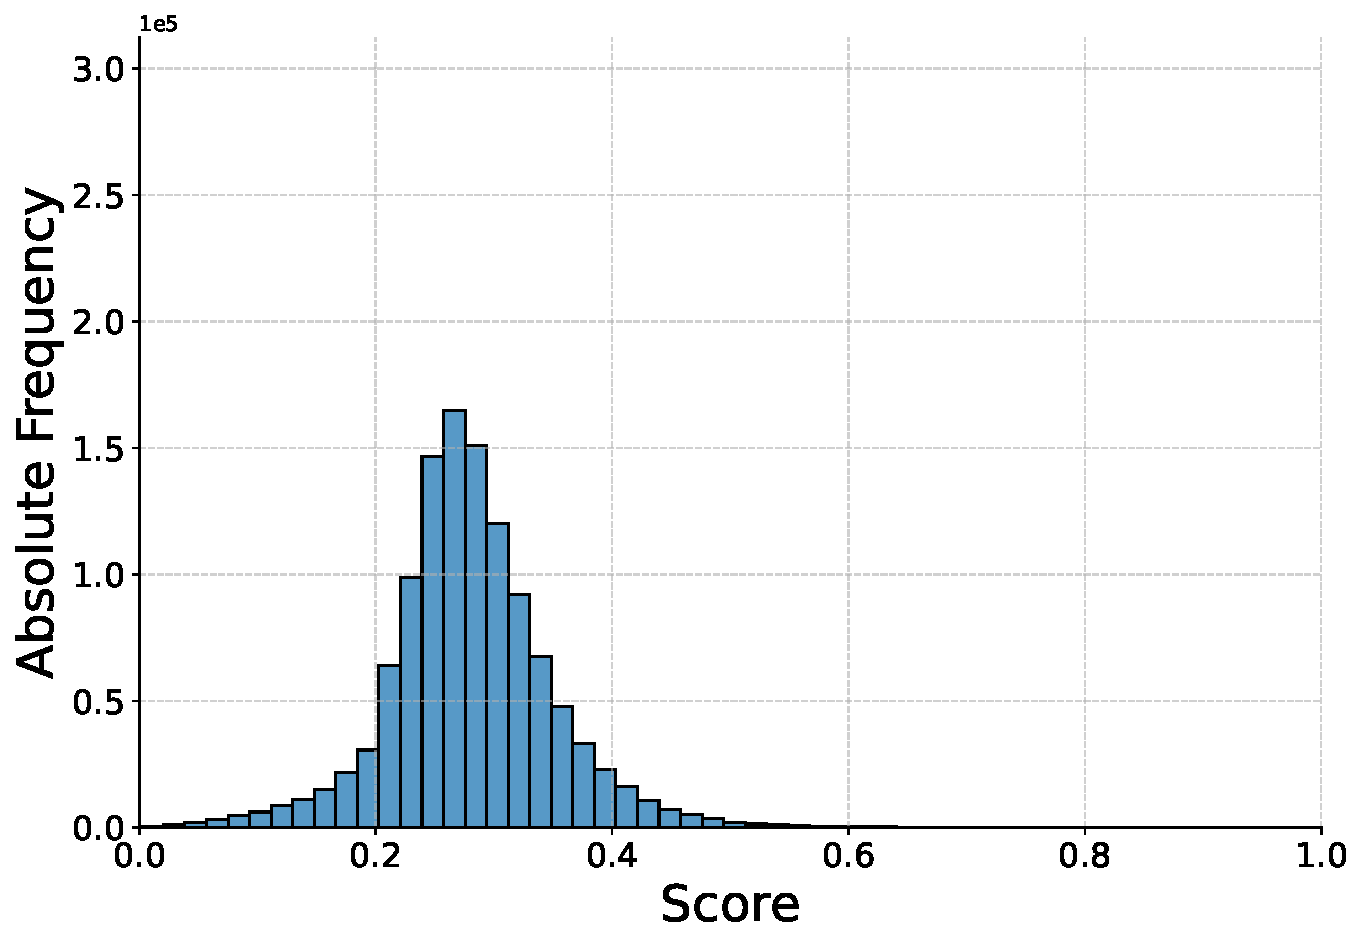
\includegraphics[width=\textwidth]{graphics/evaluation/pointwise_score_distribution_flan-t5-base.pdf}
        \label{fig:pointwise_flan-t5-base}
    \end{subfigure}

    \vspace{-0.5cm}
    \textbf{(a)} Relevance scores generated using \texttt{flan-t5-base}.
    \vspace{0.5cm}

    % Second row
    \begin{subfigure}[b]{0.49\textwidth}
        \centering
        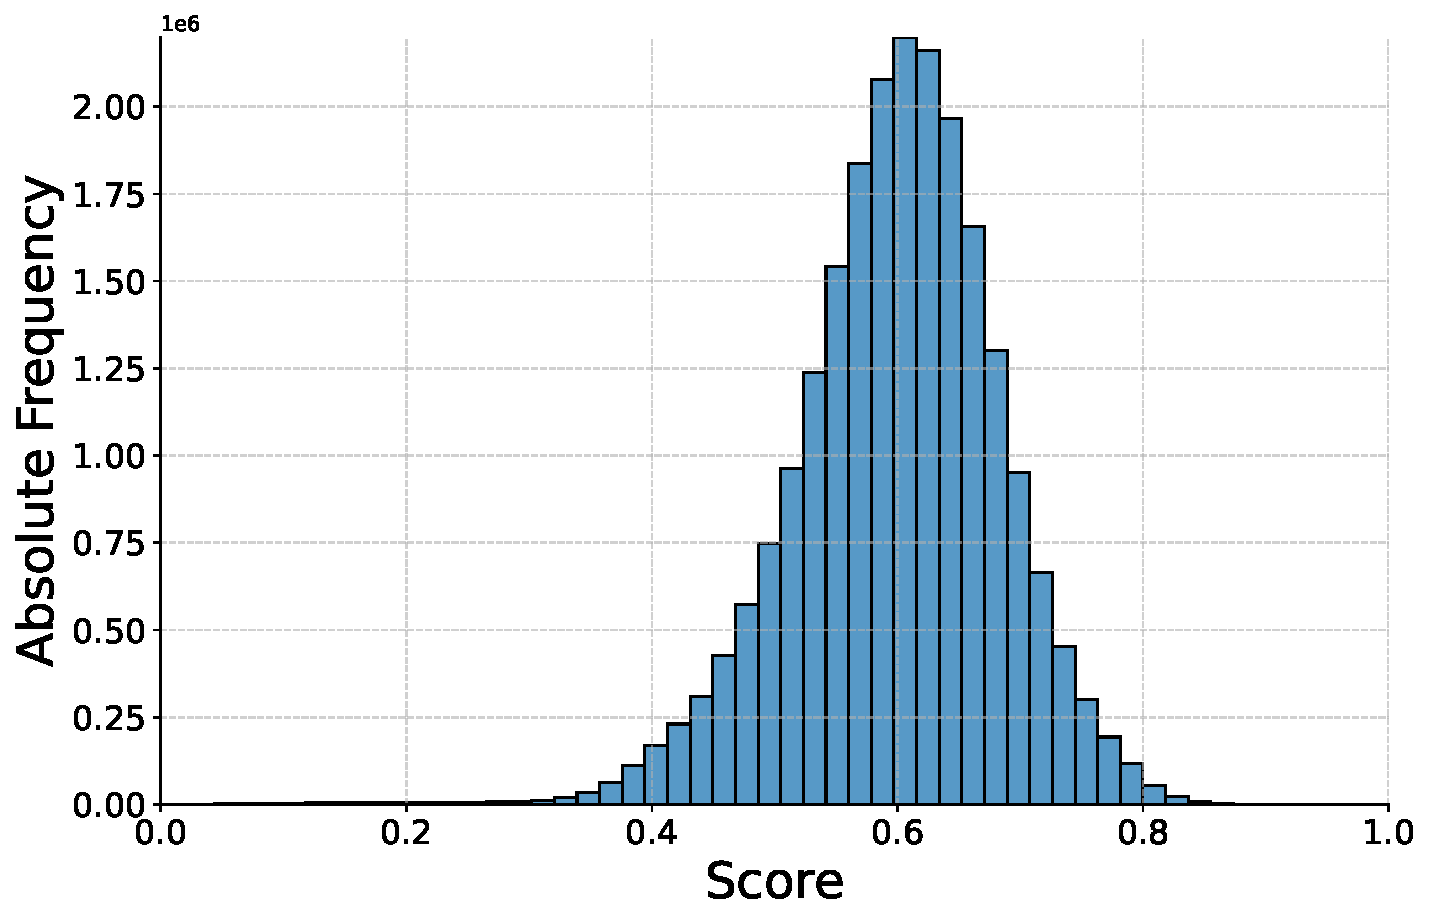
\includegraphics[width=\textwidth]{graphics/evaluation/pairwise_score_distribution_flan-t5-small.pdf}
        \label{fig:pairwise_flan-t5-small}
    \end{subfigure}
    \hfill
    \begin{subfigure}[b]{0.49\textwidth}
        \centering
        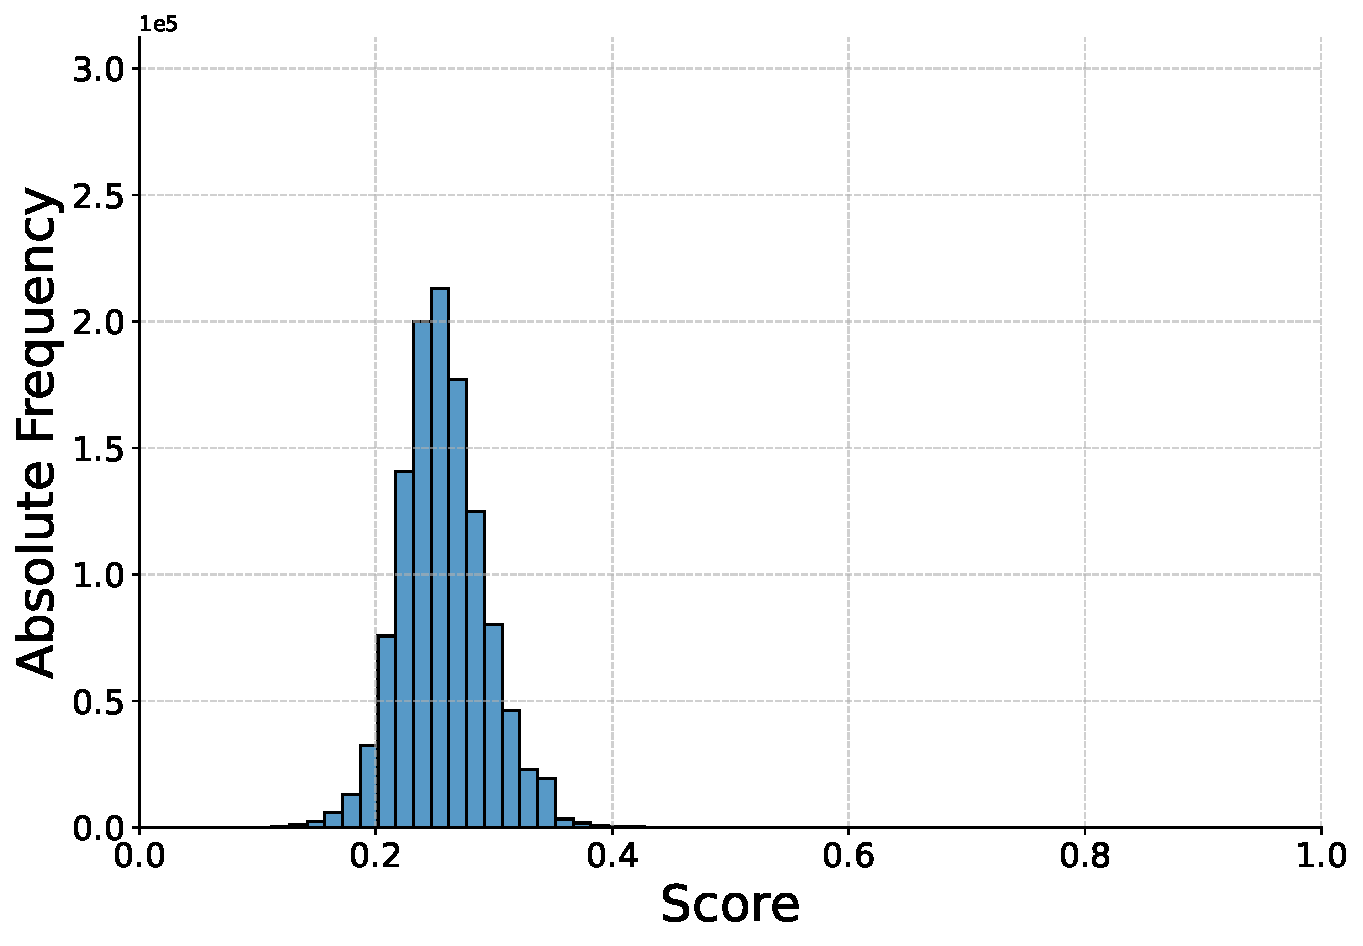
\includegraphics[width=\textwidth]{graphics/evaluation/pointwise_score_distribution_flan-t5-small.pdf}
        \label{fig:pointwise_flan-t5-small}
    \end{subfigure}

    \vspace{-0.5cm}
    \textbf{(b)} Relevance scores generated using \texttt{flan-t5-small}.
    \vspace{0.5cm}

    % Third row
    \begin{subfigure}[b]{0.49\textwidth}
        \centering
        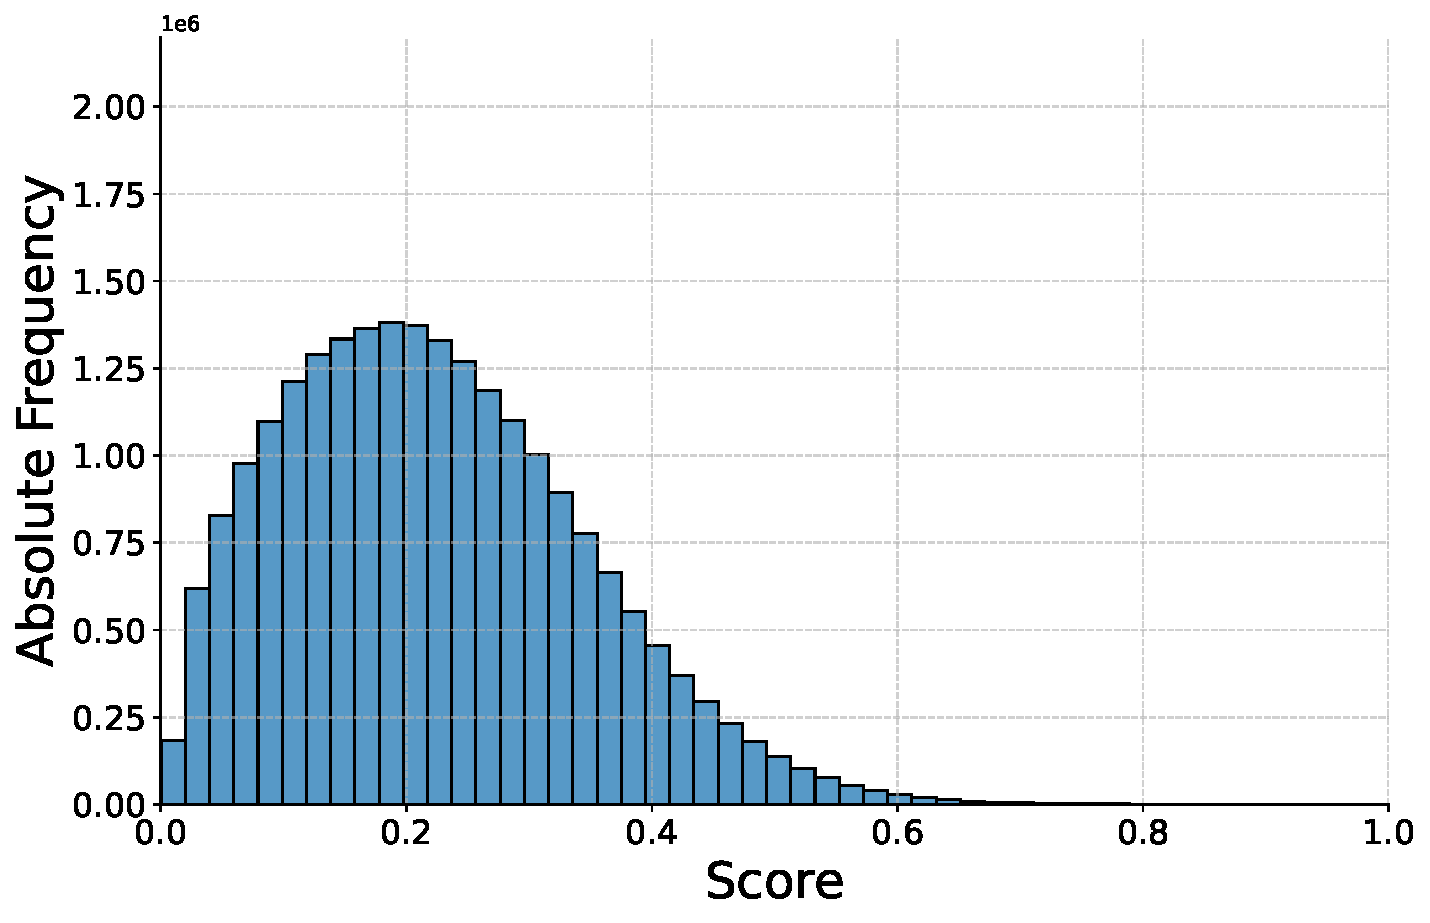
\includegraphics[width=\textwidth]{graphics/evaluation/pairwise_score_distribution_t5-small.pdf}
        \label{fig:pairwise_t5-small}
    \end{subfigure}
    \hfill
    \begin{subfigure}[b]{0.49\textwidth}
        \centering
        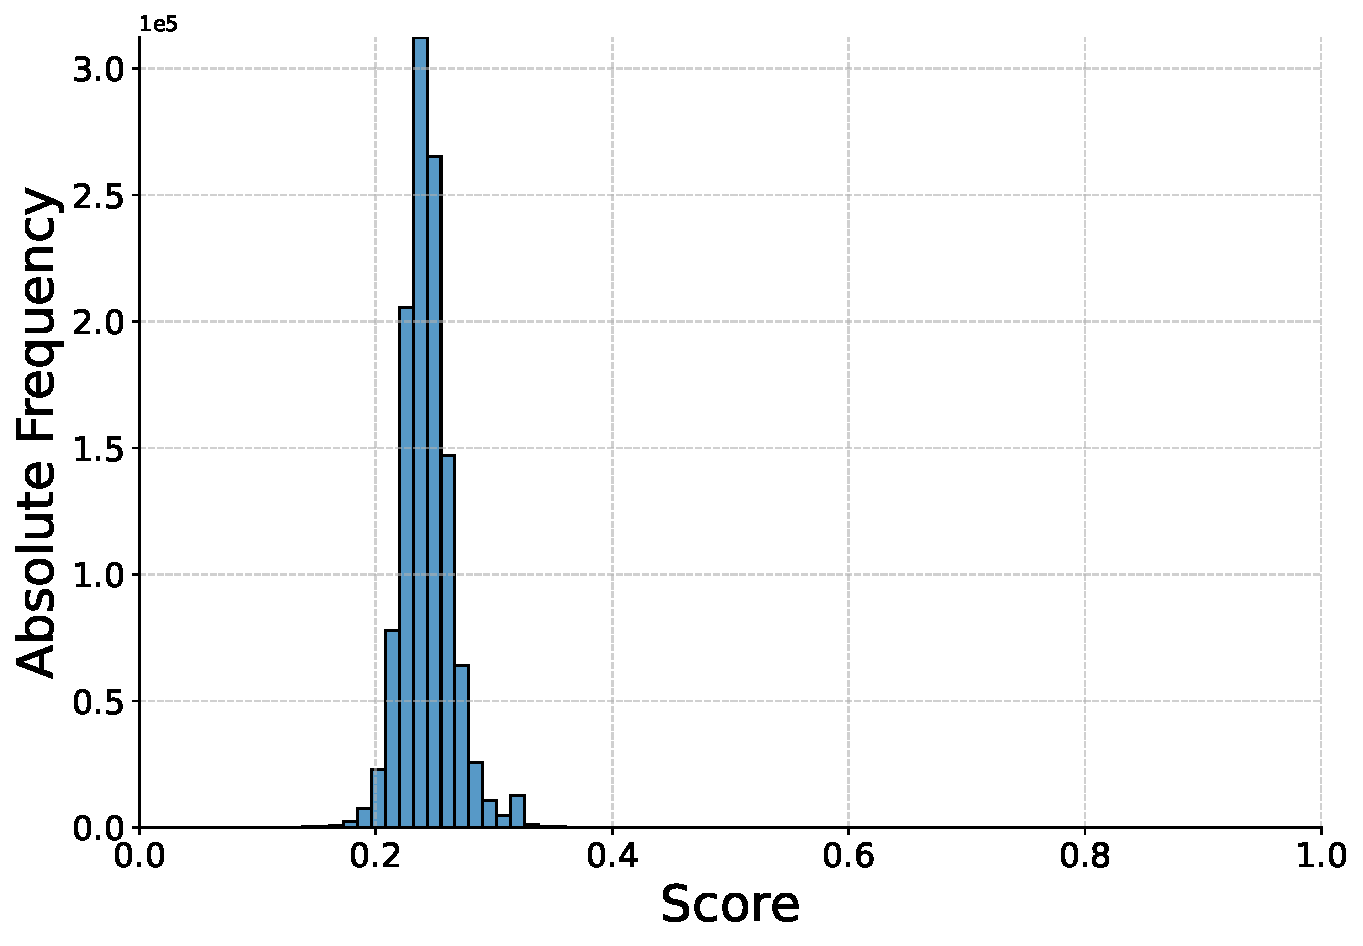
\includegraphics[width=\textwidth]{graphics/evaluation/pointwise_score_distribution_t5-small.pdf}
        \label{fig:pointwise_t5-small}
    \end{subfigure}

    \vspace{-0.5cm}
    \textbf{(c)} Relevance scores generated using \texttt{t5-small}.
    \vspace{0.5cm}

    \caption{Distributions of the inferred relevance scores over all six retrieval tasks using the pairwise and pointwise approaches with different versions of the \texttt{T5} model.}
    \label{fig:score-distributions}
\end{figure}
\\\\\\\\\\
To better analyze the rank correlation results, Figure~\ref{fig:score-distributions} visualizes the distribution of inferred relevance scores for both the pairwise and pointwise approaches across all six retrieval tasks. In general, the pairwise approach has greater score variance than the pointwise approach. This is likely because the pointwise models generate only one relevance score per passage, whereas the pairwise models compare each passage against 20 source passages, leading to more granular relevance differentiation. This also explains the overall higher number of scores in the pairwise approaches.
\\\\
When comparing pointwise models, it is evident that more advanced models introduce greater variance into the score distribution, enabling finer-grained relevance differentiation. This trend is also reflected in the rank correlation results, where \texttt{flan-t5-base} outperforms the other two models in the pointwise setting. However, the pairwise approaches exhibit significantly higher score variance overall. Looking at the distribution of the pairwise models, notable differences emerge. While \texttt{t5-small} tends to underestimate relevance scores, \texttt{flan-t5-small} assigns generally higher scores on average. In contrast, \texttt{flan-t5-base} produces the highest score variance, allowing for more effective passage differentiation. Additionally, unlike \texttt{flan-t5-small} or \texttt{t5-small}, its score distribution is more spread out rather than forming a sharp peak, suggesting a more nuanced relevance assessment. This broader score distribution is a key reason why \texttt{flan-t5-base} achieved the best overall results for both standard and greedy rank correlation. In conclusion, the ability to infer a broad spectrum of relevance scores seems to allow for better passage differentiation, reinforcing the idea that a passage's overall relevance is dependent on its weakest passage regarding that the \texttt{min} aggregation performed best.

% Transfer Pipeline to ClueWeb22/b
\subsection{Transfer Pipeline on \texttt{ClueWeb22/b}}\label{eval-pairwise-preferences-target}
\chapter{Conclusion \& Further Work}\label{conclusion}

In this thesis, I presented an approach for automatically generating new relevance judgments by leveraging existing judgments from an annotated dataset. The source dataset consisted of a document corpus and a retrieval task that provided queries and corresponding relevance judgments. To facilitate the automatic transfer of relevance judgments from the source dataset to a new document corpus, a transfer pipeline was developed. The evaluation of the pipeline in a self-transfer setting demonstrated that the pairwise approach significantly outperformed the pointwise approach in generating relevance judgments. \colorbox{red}{Waiting for Maik, pipeline to ClueWeb22/b}. This confirms that the relevance transfer process improves the quality of automatically generated relevance judgments. A  requirement for a successful transfer is that the source dataset must contain a sufficient number of high-quality relevance judgments.
\\\\
The comparison of different versions of the \texttt{T5} model indicated that more fine-tuned models achieved higher rank correlations. It is therefore likely that using an even larger version of \texttt{FLAN-T5} with more parameters would achieve even better relevance predictions. Future work could also explore benchmarking and comparing entirely different large language models for performing pairwise preference inference. Another key component of the transfer pipeline was the \texttt{Union opd.\ 100} approach, which was found to be the most effective candidate selection method in this thesis. However, further research could refine the process of selecting likely relevant candidate documents. The nearest neighbor approach already demonstrated strong performance, and combining it with the naive selection approach even increased recall, but at the cost of a larger candidate set. A more fine-tuned version of this approach could be developed to further optimize relevance transfer.


% \\\\
% The pipeline involved several key steps: preprocessing the source dataset, identifying candidate documents from the target corpus, and generating new relevance judgments. For each query in the retrieval task, selected candidate documents were segmented into passages. Each passage was then compared against the 15 most relevant and 5 least relevant passages from the source dataset for the same query. A large language model performed pairwise preference comparisons to assess how relevant each target passage was relative to the known source passage. These comparisons were then aggregated to assign a final relevance score to each target document.

000\appendix
\chapter{Greedy Evaluation}\label{app:greedy-evaluation}

\begin{table}[t]
    \centering
    \caption{Average rank correlations between the assigned passage scores and the original relevance judgments across all queries of a retrieval task, reported using the \texttt{greedy} version of Kendall's $\tau$ and Spearman's $\rho$.}
    \label{tab:app:passage-scoring}
    \resizebox{\textwidth}{!}{%
    \renewcommand{\arraystretch}{1.2}
    \begin{tabular}{clcccccccccccccc}
        \toprule
        \multicolumn{2}{c}{\textbf{Retrieval Model}} & \multicolumn{2}{c}{\textbf{Touché 20}} & \multicolumn{2}{c}{\textbf{Robust04}} & \multicolumn{2}{c}{\textbf{TREC-7}} & \multicolumn{2}{c}{\textbf{TREC-8}} & \multicolumn{2}{c}{\textbf{TREC-19 DL}} & \multicolumn{2}{c}{\textbf{TREC-20 DL}} & \multicolumn{2}{c}{\textbf{Avg.}} \\
        \cmidrule(lr){3-4} \cmidrule(lr){5-6} \cmidrule(lr){7-8} \cmidrule(lr){9-10} \cmidrule(lr){11-12} \cmidrule(lr){13-14} \cmidrule(lr){15-16}
                                                   & & $\tau$ & $\rho$ & $\tau$ & $\rho$ & $\tau$ & $\rho$ & $\tau$ & $\rho$ & $\tau$ & $\rho$ & $\tau$ & $\rho$ & $\tau$ & $\rho$ \\
        \midrule
        \multirow{10}{*}{\rotatebox{90}{\texttt{ndcg@10}}}
            & BM25         & 0.886 & 0.908 & 0.951 & 0.957 & 0.954 & 0.954 & 0.971 & 0.971 & 0.800 & 0.837 & 0.843 & 0.874 & 0.901 & 0.917 \\
            & DFR\_BM25    & 0.886 & 0.909 & 0.950 & 0.956 & 0.952 & 0.952 & 0.972 & 0.972 & 0.803 & 0.840 & 0.845 & 0.877 & 0.901 & 0.918 \\
            & DFIZ         & 0.865 & 0.888 & 0.953 & 0.959 & 0.957 & 0.957 & 0.970 & 0.970 & 0.805 & 0.841 & 0.839 & 0.871 & 0.898 & 0.914 \\
            & DLH          & 0.912 & 0.932 & 0.950 & 0.956 & 0.954 & 0.954 & 0.973 & 0.973 & 0.804 & 0.841 & 0.840 & 0.872 & 0.905 & 0.921 \\
            & DPH          & 0.866 & 0.890 & 0.951 & 0.957 & 0.955 & 0.955 & 0.971 & 0.971 & 0.794 & 0.832 & 0.838 & 0.869 & 0.896 & 0.912 \\
            & DirichletLM  & 0.756 & 0.781 & 0.951 & 0.958 & 0.958 & 0.958 & 0.966 & 0.966 & 0.790 & 0.826 & 0.824 & 0.857 & 0.874 & 0.891 \\
            & Hiemstra\_LM & 0.923 & 0.944 & 0.952 & 0.958 & 0.956 & 0.956 & 0.971 & 0.971 & 0.805 & 0.841 & 0.842 & 0.874 & \textbf{0.908} & \textbf{0.924} \\
            & LGD          & 0.890 & 0.914 & 0.952 & 0.958 & 0.959 & 0.959 & 0.968 & 0.968 & 0.806 & 0.842 & 0.843 & 0.874 & 0.903 & 0.919 \\
            & PL2          & 0.888 & 0.912 & 0.948 & 0.954 & 0.952 & 0.952 & 0.973 & 0.973 & 0.798 & 0.835 & 0.849 & 0.880 & 0.901 & 0.918 \\
            & TF\_IDF      & 0.892 & 0.916 & 0.949 & 0.955 & 0.953 & 0.953 & 0.969 & 0.969 & 0.803 & 0.840 & 0.844 & 0.876 & 0.902 & 0.918 \\
        \midrule
        \multirow{10}{*}{\rotatebox{90}{\texttt{precision@10}}}
            & BM25         & 0.797 & 0.830 & 0.880 & 0.890 & 0.878 & 0.878 & 0.901 & 0.901 & 0.693 & 0.744 & 0.732 & 0.776 & 0.814 & 0.837 \\
            & DFR\_BM25    & 0.801 & 0.833 & 0.879 & 0.889 & 0.877 & 0.877 & 0.902 & 0.902 & 0.692 & 0.743 & 0.733 & 0.777 & 0.814 & 0.837 \\
            & DFIZ         & 0.768 & 0.801 & 0.876 & 0.886 & 0.876 & 0.876 & 0.889 & 0.889 & 0.699 & 0.748 & 0.732 & 0.777 & 0.807 & 0.829 \\
            & DLH          & 0.829 & 0.864 & 0.890 & 0.900 & 0.887 & 0.887 & 0.924 & 0.924 & 0.700 & 0.750 & 0.733 & 0.777 & 0.827 & 0.850 \\
            & DPH          & 0.788 & 0.822 & 0.876 & 0.886 & 0.872 & 0.872 & 0.893 & 0.893 & 0.690 & 0.740 & 0.731 & 0.775 & 0.808 & 0.831 \\
            & DirichletLM  & 0.687 & 0.716 & 0.867 & 0.877 & 0.869 & 0.869 & 0.879 & 0.879 & 0.683 & 0.731 & 0.735 & 0.778 & 0.787 & 0.808 \\
            & Hiemstra\_LM & 0.845 & 0.883 & 0.887 & 0.897 & 0.885 & 0.885 & 0.916 & 0.916 & 0.698 & 0.746 & 0.738 & 0.782 & \textbf{0.828} & \textbf{0.851} \\
            & LGD          & 0.804 & 0.840 & 0.873 & 0.883 & 0.873 & 0.873 & 0.882 & 0.882 & 0.695 & 0.744 & 0.735 & 0.778 & 0.810 & 0.834 \\
            & PL2          & 0.805 & 0.838 & 0.883 & 0.893 & 0.886 & 0.886 & 0.917 & 0.917 & 0.688 & 0.738 & 0.734 & 0.777 & 0.819 & 0.842 \\
            & TF\_IDF      & 0.801 & 0.834 & 0.881 & 0.891 & 0.878 & 0.878 & 0.902 & 0.902 & 0.694 & 0.745 & 0.732 & 0.775 & 0.815 & 0.837 \\

        \bottomrule
    \end{tabular}}
    \renewcommand{\arraystretch}{1.0}
\end{table}


% Bibliography
\bibliographystyle{plainnat} % requires package natbib. An alternative is apalike
\bibliography{literature}    % load file literature.bib

\end{document}

